%%%%%%%%%%%%%%%%%%%%%%%%%%%%%%%%%%%%%%%%%
% Beamer Presentation
% LaTeX Template
% Version 2.0 (March 8, 2022)
%
% This template originates from:
% https://www.LaTeXTemplates.com
%
% Author:
% Vel (vel@latextemplates.com)
%
% License:
% CC BY-NC-SA 4.0 (https://creativecommons.org/licenses/by-nc-sa/4.0/)
%
%%%%%%%%%%%%%%%%%%%%%%%%%%%%%%%%%%%%%%%%%

%----------------------------------------------------------------------------------------
%	PACKAGES AND OTHER DOCUMENT CONFIGURATIONS
%----------------------------------------------------------------------------------------





\documentclass[
	10pt, % Set the default font size, options include: 8pt, 9pt, 10pt, 11pt, 12pt, 14pt, 17pt, 20pt
	%t, % Uncomment to vertically align all slide content to the top of the slide, rather than the default centered
	%aspectratio=169, % Uncomment to set the aspect ratio to a 16:9 ratio which matches the aspect ratio of 1080p and 4K screens and projectors
]{beamer}

\graphicspath{{figures/}{./}} % Specifies where to look for included images (trailing slash required)




\usepackage{booktabs} % Allows the use of \toprule, \midrule and \bottomrule for better rules in tables
\usepackage{multimedia}


\usepackage{siunitx}
\usepackage{hyperref}
\usepackage{outlines}
\usepackage{float}
% \usepackage{caption}
\usepackage{subcaption}
\usepackage{cases}

\renewcommand{\vec}[1]{\mathbf{#1}} % bold text instead of arrow




% \usepackage[backend=bibtex, 
%             style=phys, 
%             biblabel=brackets]{biblatex}



%----------------------------------------------------------------------------------------
%	THEME
%----------------------------------------------------------------------------------------

\usetheme{Madrid} %%%
\usefonttheme{default} % Typeset using the default sans serif font
% \usecolortheme{dolphin}
\definecolor{myblue}{RGB}{138,162,247}
\setbeamercolor{structure}{fg=myblue}
\setbeamercolor{section in head/foot}{bg=myblue}


%\usepackage{mathptmx} % Use the Times font for serif text
\usepackage{palatino} % Use the Palatino font for serif text

%\usepackage{helvet} % Use the Helvetica font for sans serif text
\usepackage[default]{opensans} % Use the Open Sans font for sans serif text
%\usepackage[default]{FiraSans} % Use the Fira Sans font for sans serif text
%\usepackage[default]{lato} % Use the Lato font for sans serif text

\useinnertheme{circles}
\useoutertheme{default}

% \setbeamertemplate{footline} % Uncomment this line to remove the footer line in all slides
% \setbeamertemplate{footline}[page number] % Uncomment this line to replace the footer line in all slides with a simple slide count
\setbeamertemplate{navigation symbols}{} % Uncomment this line to remove the navigation symbols from the bottom of all slides


% \usepackage{textpos} 
% \addtobeamertemplate{frametitle}{}{%
%     \begin{textblock*}{100mm}(0.96\textwidth,-0.85cm)
%         
\includegraphics[height=0.8cm,width=0.8cm]{UiO_segl_pos-eps-converted-to.pdf}
%     \end{textblock*}}


%----------------------------------------------------------------------------------------
%	PRESENTATION INFORMATION
%----------------------------------------------------------------------------------------

\title[Predicting Graphene Kirigami Friction]{Predicting Frictional Properties of Graphene Kirigami Using Molecular Dynamics and Neural Networks}
\subtitle{Designs for a negative friction coefficient} 
\author[Mikkel Metzsch Jensen]{Mikkel Metzsch Jensen}
\institute[UiO]{University of Oslo}
\date[Juni 02, 2023]{Juni 02, 2023}

\titlegraphic{\flushleft
\includegraphics[width=0.5\textwidth]{figures/MN_FYSISK_A_ENG.pdf}}

% \titlegraphic{\vspace{4cm}\flushright\includegraphics[width=2cm,height=2cm]{example-image-a}} 


\setbeamertemplate{bibliography item}{\insertbiblabel}
\usepackage[backend=bibtex, 
            style=phys, 
            biblabel=brackets]{biblatex}
\addbibresource{bibliography.bib}




%----------------------------------------------------------------------------------------
\begin{document}

%----------------------------------------------------------------------------------------
%	TITLE SLIDE
%----------------------------------------------------------------------------------------

\begin{frame}
	\titlepage % Output the title slide, automatically created using the text entered in the PRESENTATION INFORMATION block above
\end{frame}

%----------------------------------------------------------------------------------------
%	BODY
%----------------------------------------------------------------------------------------

\begin{frame}{Outline}
    \tableofcontents
\end{frame}
%
%%% New frame %%%
%
\section{Introduction} %%%%%%%%%%%%%%%%%%%%%%%%%%%%%%%%%%%%%%%%%%%%%%%%%%%%%%%%%%%%%
\subsection{Thesis overview}
\begin{frame}{Overview}
	\framesubtitle{Three main parts}
	\begin{enumerate}
		\setlength\itemsep{1em}
		\item \textbf{Sheet kirigami}: Alter a graphene sheet using atomic scale cuts and stretching
		\item \textbf{Forward simulation}: Calculate the frictional properties of the sheet using MD simulations
		\item \textbf{Accelerated search}: Use machine learning to replace the MD simulations and perform an accelerated search for new designs
	\end{enumerate}
	\vspace{2mm}
	
	Can we control the frictional properties of a graphene sheet using this technique?
	% \begin{itemize}
	% 	\item Can we utilize a coupling between load and stretch?
	% 	\item Negative friction coefficients
	% \end{itemize}
	
\end{frame}
%
%%% New frame %%%
%
\subsection{Motivation}
\begin{frame}{Motivation}
	\begin{itemize}
		\item Kirigami: Variation of origami with cuts permitted
		\item Desgins: Macroscale $\to$ nanoscale
	\end{itemize}
	\vspace*{10px}

	\begin{figure}
		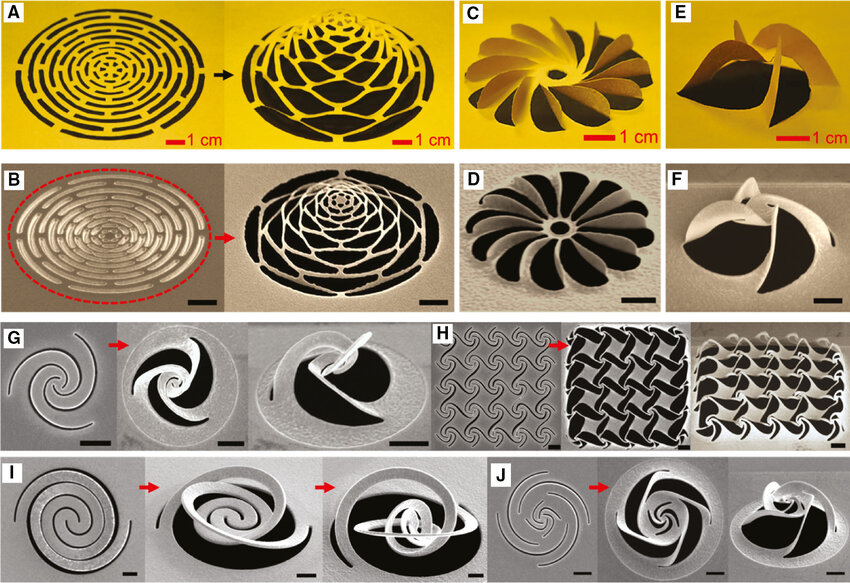
\includegraphics[height=0.55\textheight]{figures/kirigami_example.jpg}
		\caption{Example of macroscale Kirigami designs implemented on a nanoscale using a focused ion beam (FIB). Black scale bars: \SI{1}{\mu m}. Reproduced from~\cite{Li_2018}.}
	\end{figure}	
\end{frame}
%
%%% New frame %%%
%
\begin{frame}{Motivation}
	\framesubtitle{Out-of-plane buckling}
	\vspace{0.5cm}
	
	\begin{itemize}
		\item Hanakata et al. \cite{Hanakata_2018,Hanakata_2020} found out-of-plane buckling with Kirigami designs
		\item Surface properties are predicted to be important for friction properties
		\begin{itemize}
			\item Asperity theory: Contact area
			\item Frenkel–Kontorova models: Commensurability
		\end{itemize}
	\end{itemize}
	% \vspace{1cm}

	\begin{figure}[H]
		\centering
		\begin{subfigure}[b]{0.49\textwidth}
			\centering
			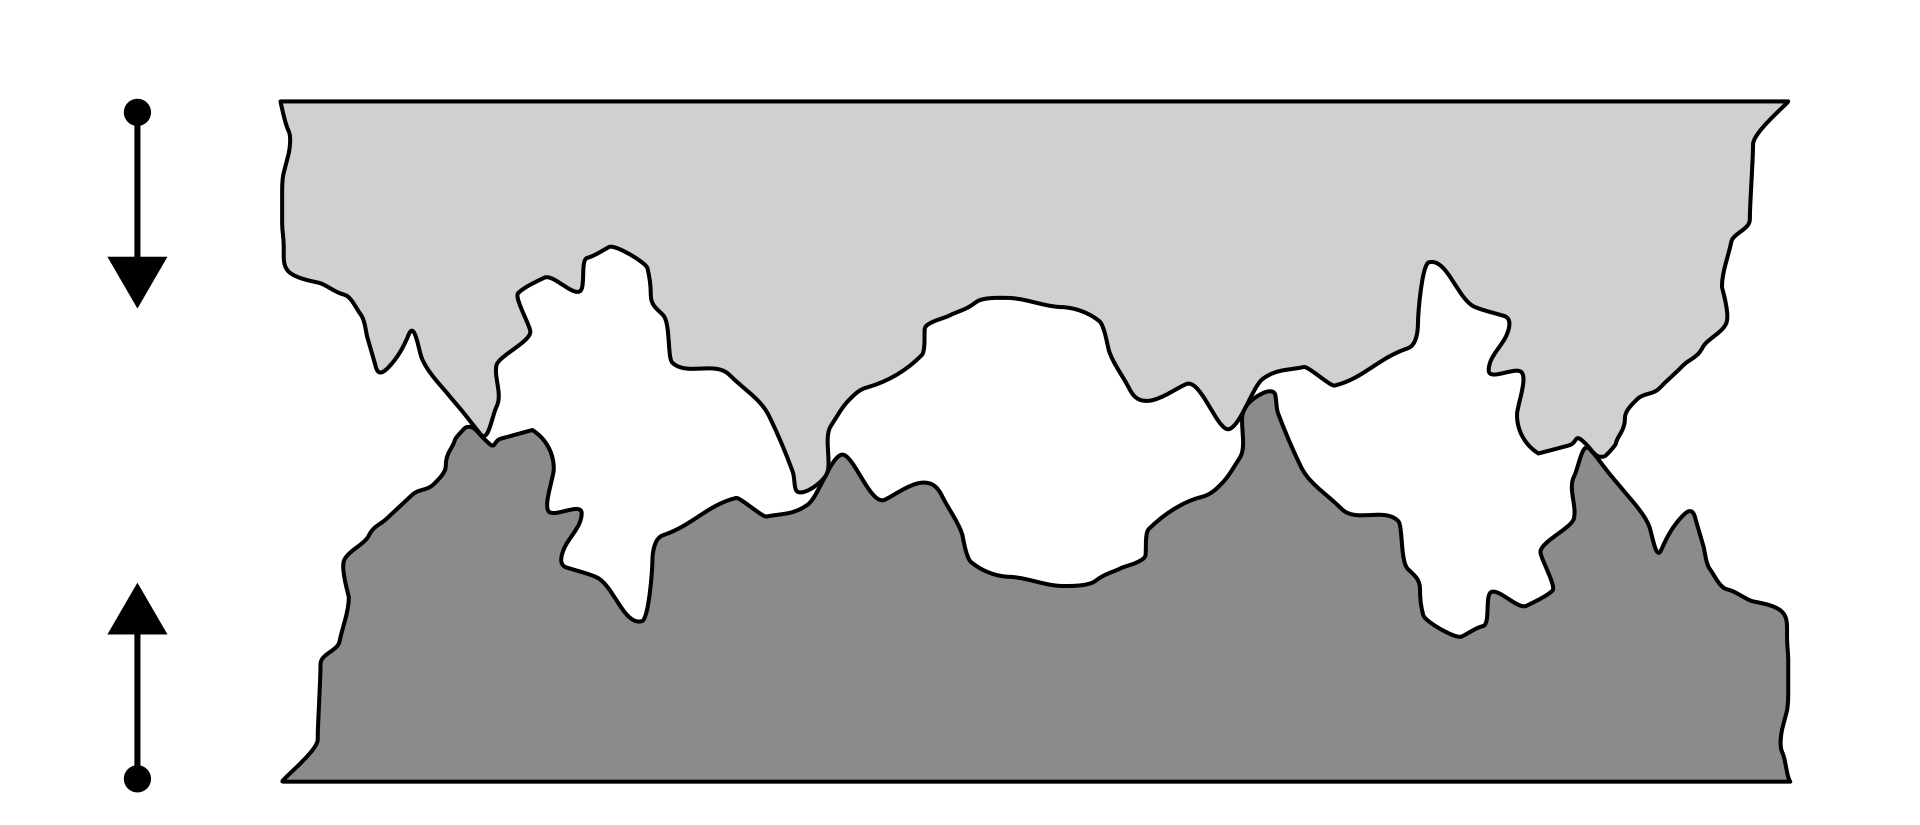
\includegraphics[width=\textwidth]{../thesis/figures/theory/asperities_top.png}
			\caption{Small load.}
			\label{fig:asp_left}
		\end{subfigure}
		\hfill
		\begin{subfigure}[b]{0.49\textwidth}
			\centering
			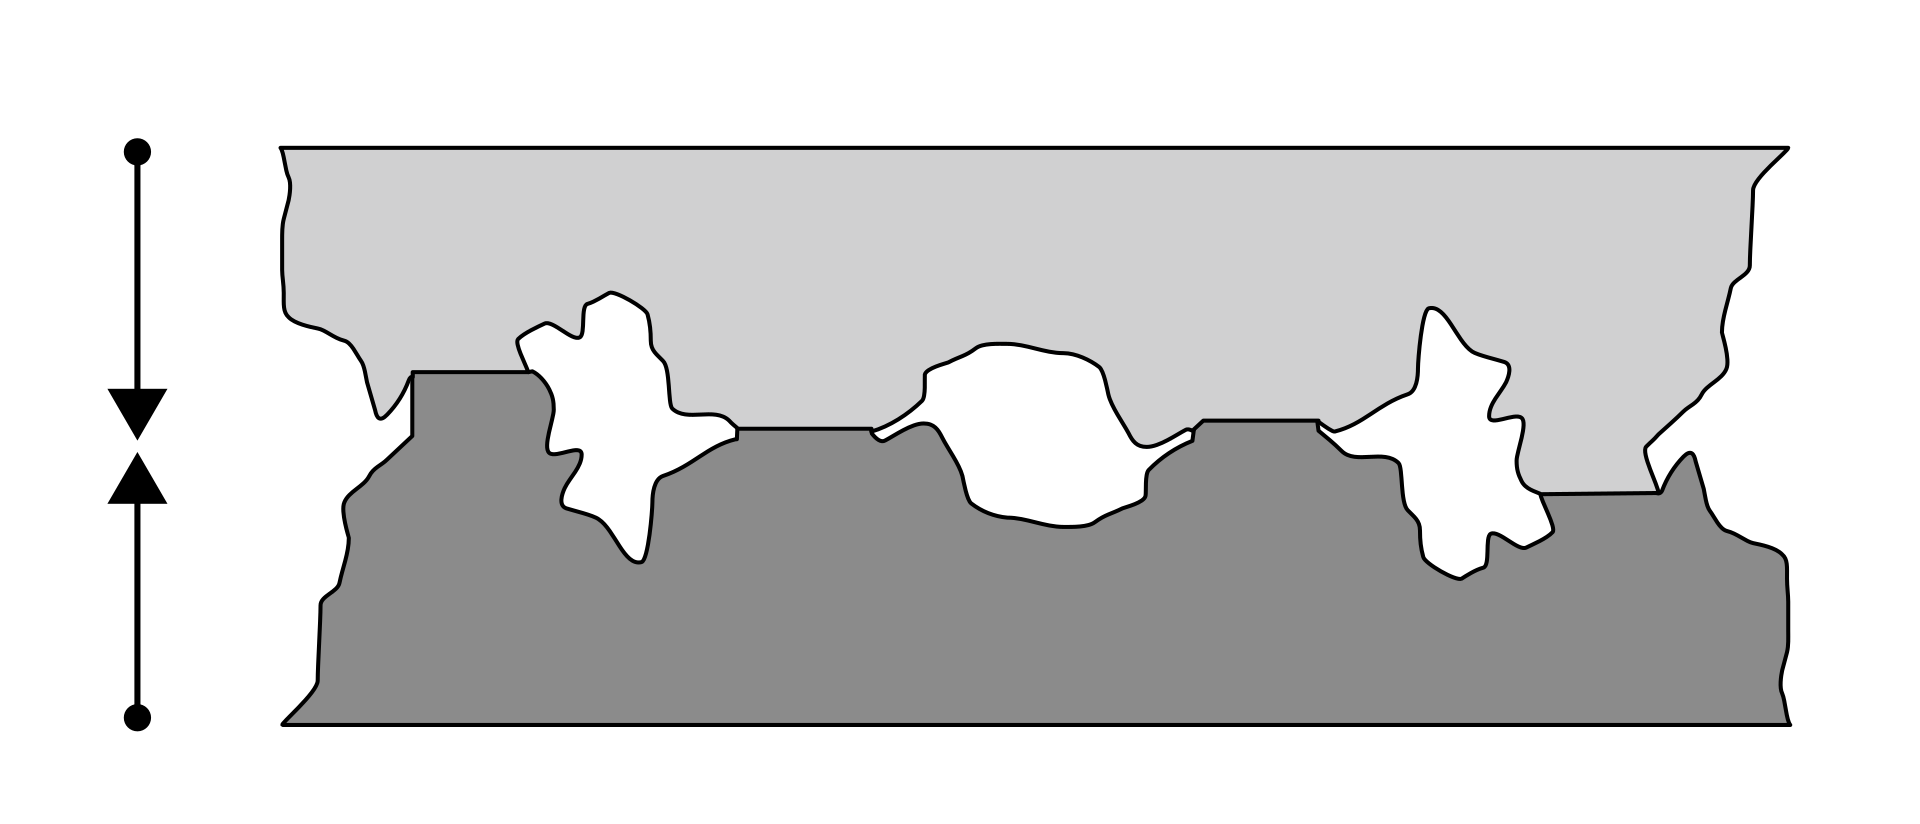
\includegraphics[width=\textwidth]{../thesis/figures/theory/asperities_bottom.png}
			\caption{High load.}
			\label{fig:asp_right}
		\end{subfigure}
		\caption{Reproduced from~\cite{wiki:asperities}.}
	\end{figure}
\end{frame}
%
%%% New frame %%%
%
\begin{frame}{Motivation}
\framesubtitle{Contact area and commensurability}
\begin{figure}[H]
	\centering
	\begin{subfigure}[b]{0.46\textwidth}
		\centering
		\includegraphics[width=\textwidth]{figures/nano_asperity_contact.png}
		\caption{Numerical MD results using an amorphous carbon tip and a diamond sample. Reproduced from~\cite{mo_friction_2009} with permission from the Springer Nature.}
	\end{subfigure}
	\hfill
	\begin{subfigure}[b]{0.49\textwidth}
		\centering
		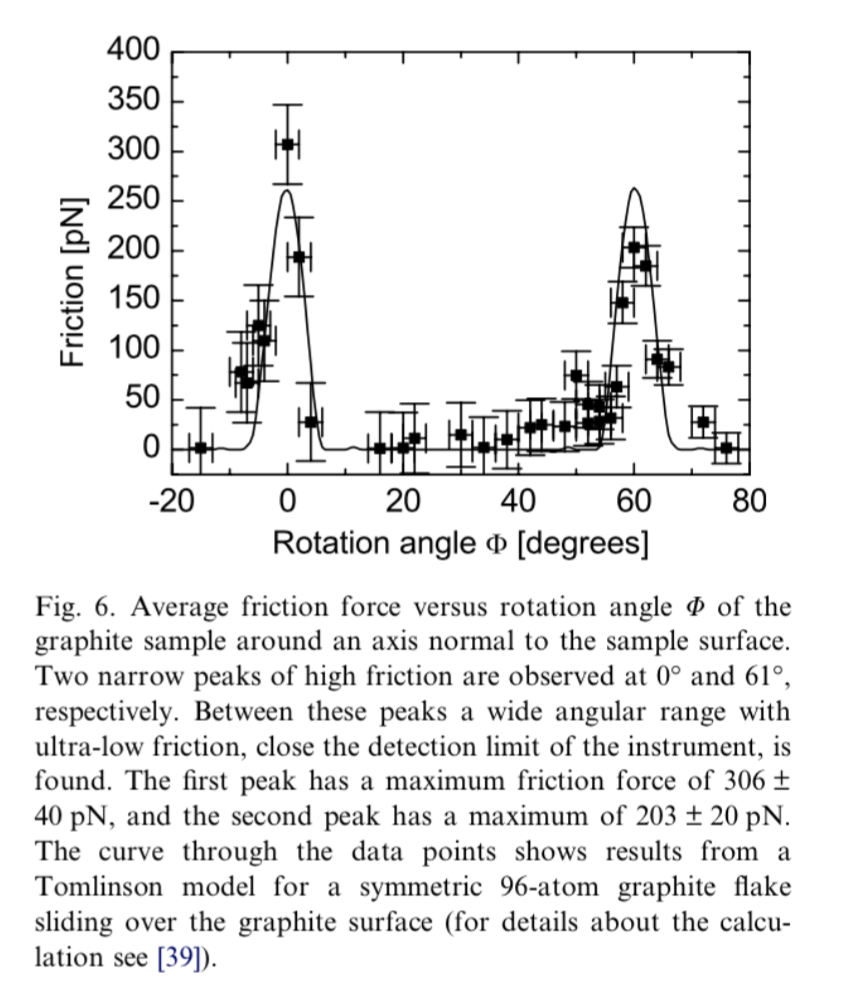
\includegraphics[width=\textwidth]{../thesis/figures/theory/graphene_rot.png}
		\caption{Experimental results of a graphene sheet sliding on graphite. Adapted from~\cite{DIENWIEBEL2005197}, reproduced from~\cite{Vanossi_2013} with permission from the American Physical Society.}
	\end{subfigure}
	% \caption{}
\end{figure}
\end{frame}
%
%%% New frame %%%
%
\subsection{System setup}
\begin{frame}{Outline}
    \tableofcontents[currentsection]
\end{frame}

\section{Creating a graphene Kirigami system} %%%%%%%%%%%%%%%%%%%%%%%%%%%%%%%%%%%%%%%%%%%%%%%%%%%%%%%%%%%%%
\begin{frame}{Creating a graphene Kirigami system}
\framesubtitle{System setup}
	\begin{figure}
		\centering    
		\movie[open,loop,repeat]{\includegraphics[height=0.5\textwidth, keepaspectratio]{figures/sim_parts.png}}{figures/sim_parts.mov}
		\caption{Graphene sheet on a silicon substrate. Blue: Substrate, Red: Inner sheet, Grey: Pull blocks. }
	\end{figure} 
\end{frame}
%
%%% New frame %%%
%
\begin{frame}{Creating a graphene Kirigami system}
\framesubtitle{System setup}
	System size = ???

	\begin{figure}[H]
		\centering
		\begin{subfigure}[b]{0.5\textwidth}
			\centering
			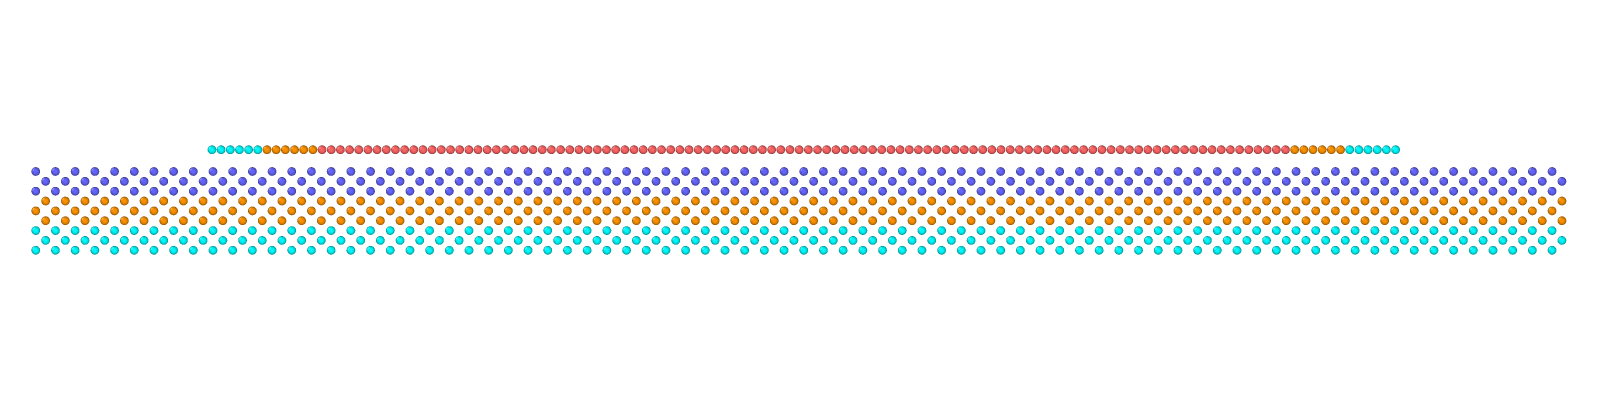
\includegraphics[width=\textwidth]{../thesis/figures/system/system_sideview.png}
			\caption{Side view.}
		\end{subfigure}
		\begin{subfigure}[b]{0.5\textwidth}
			\centering
			\includegraphics[width=\textwidth]{../thesis/figures/system/system_topview_anno.png}
			\caption{Top view.}
		\end{subfigure}
		%    \caption{System configuration colorized to indicate NVE parts (red), thermostat parts (green) and rigid parts (blue). (a) Side view showing the sheet on top of the substrate. (b) Top view showing only the sheet.}
		%    \label{fig:system}
	\end{figure}
\end{frame}
%
%%% New frame %%%
%
\subsection{Kirigami}
\begin{frame}{Creating a graphene Kirigami system}
	\framesubtitle{Sheet Kirigami}

	Primitive lattice vectors
	\begin{align*}
		&\vec{a_1} = a \left(\frac{\sqrt{3}}{2}, -\frac{1}{2}\right)&  &\vec{a_2} = a \left(\frac{\sqrt{3}}{2}, \frac{1}{2}\right),& &|\vec{a_1}| = |\vec{a_2}| = a = \SI{2.46}{\text{Å}}.& 
	\end{align*}
	
	\begin{columns} 
		\begin{column}{.4\textwidth}
			Basis
			\begin{align*}
				\Big\{\Big(0,0\Big), \frac{a}{2}\Big(\frac{1}{\sqrt{3}}, 1 \Big) \Big\}.
			  \end{align*}
			Interatomic distance
			\begin{align*}
				\left|\left|\frac{a}{2}\Big(\frac{1}{\sqrt{3}}, 1 \Big)\right|\right| \approx \SI{1.42}{\text{Å}}.
			\end{align*}
		\end{column}
		\begin{column}{.6\textwidth}
			\begin{figure}[H]
				\centering
				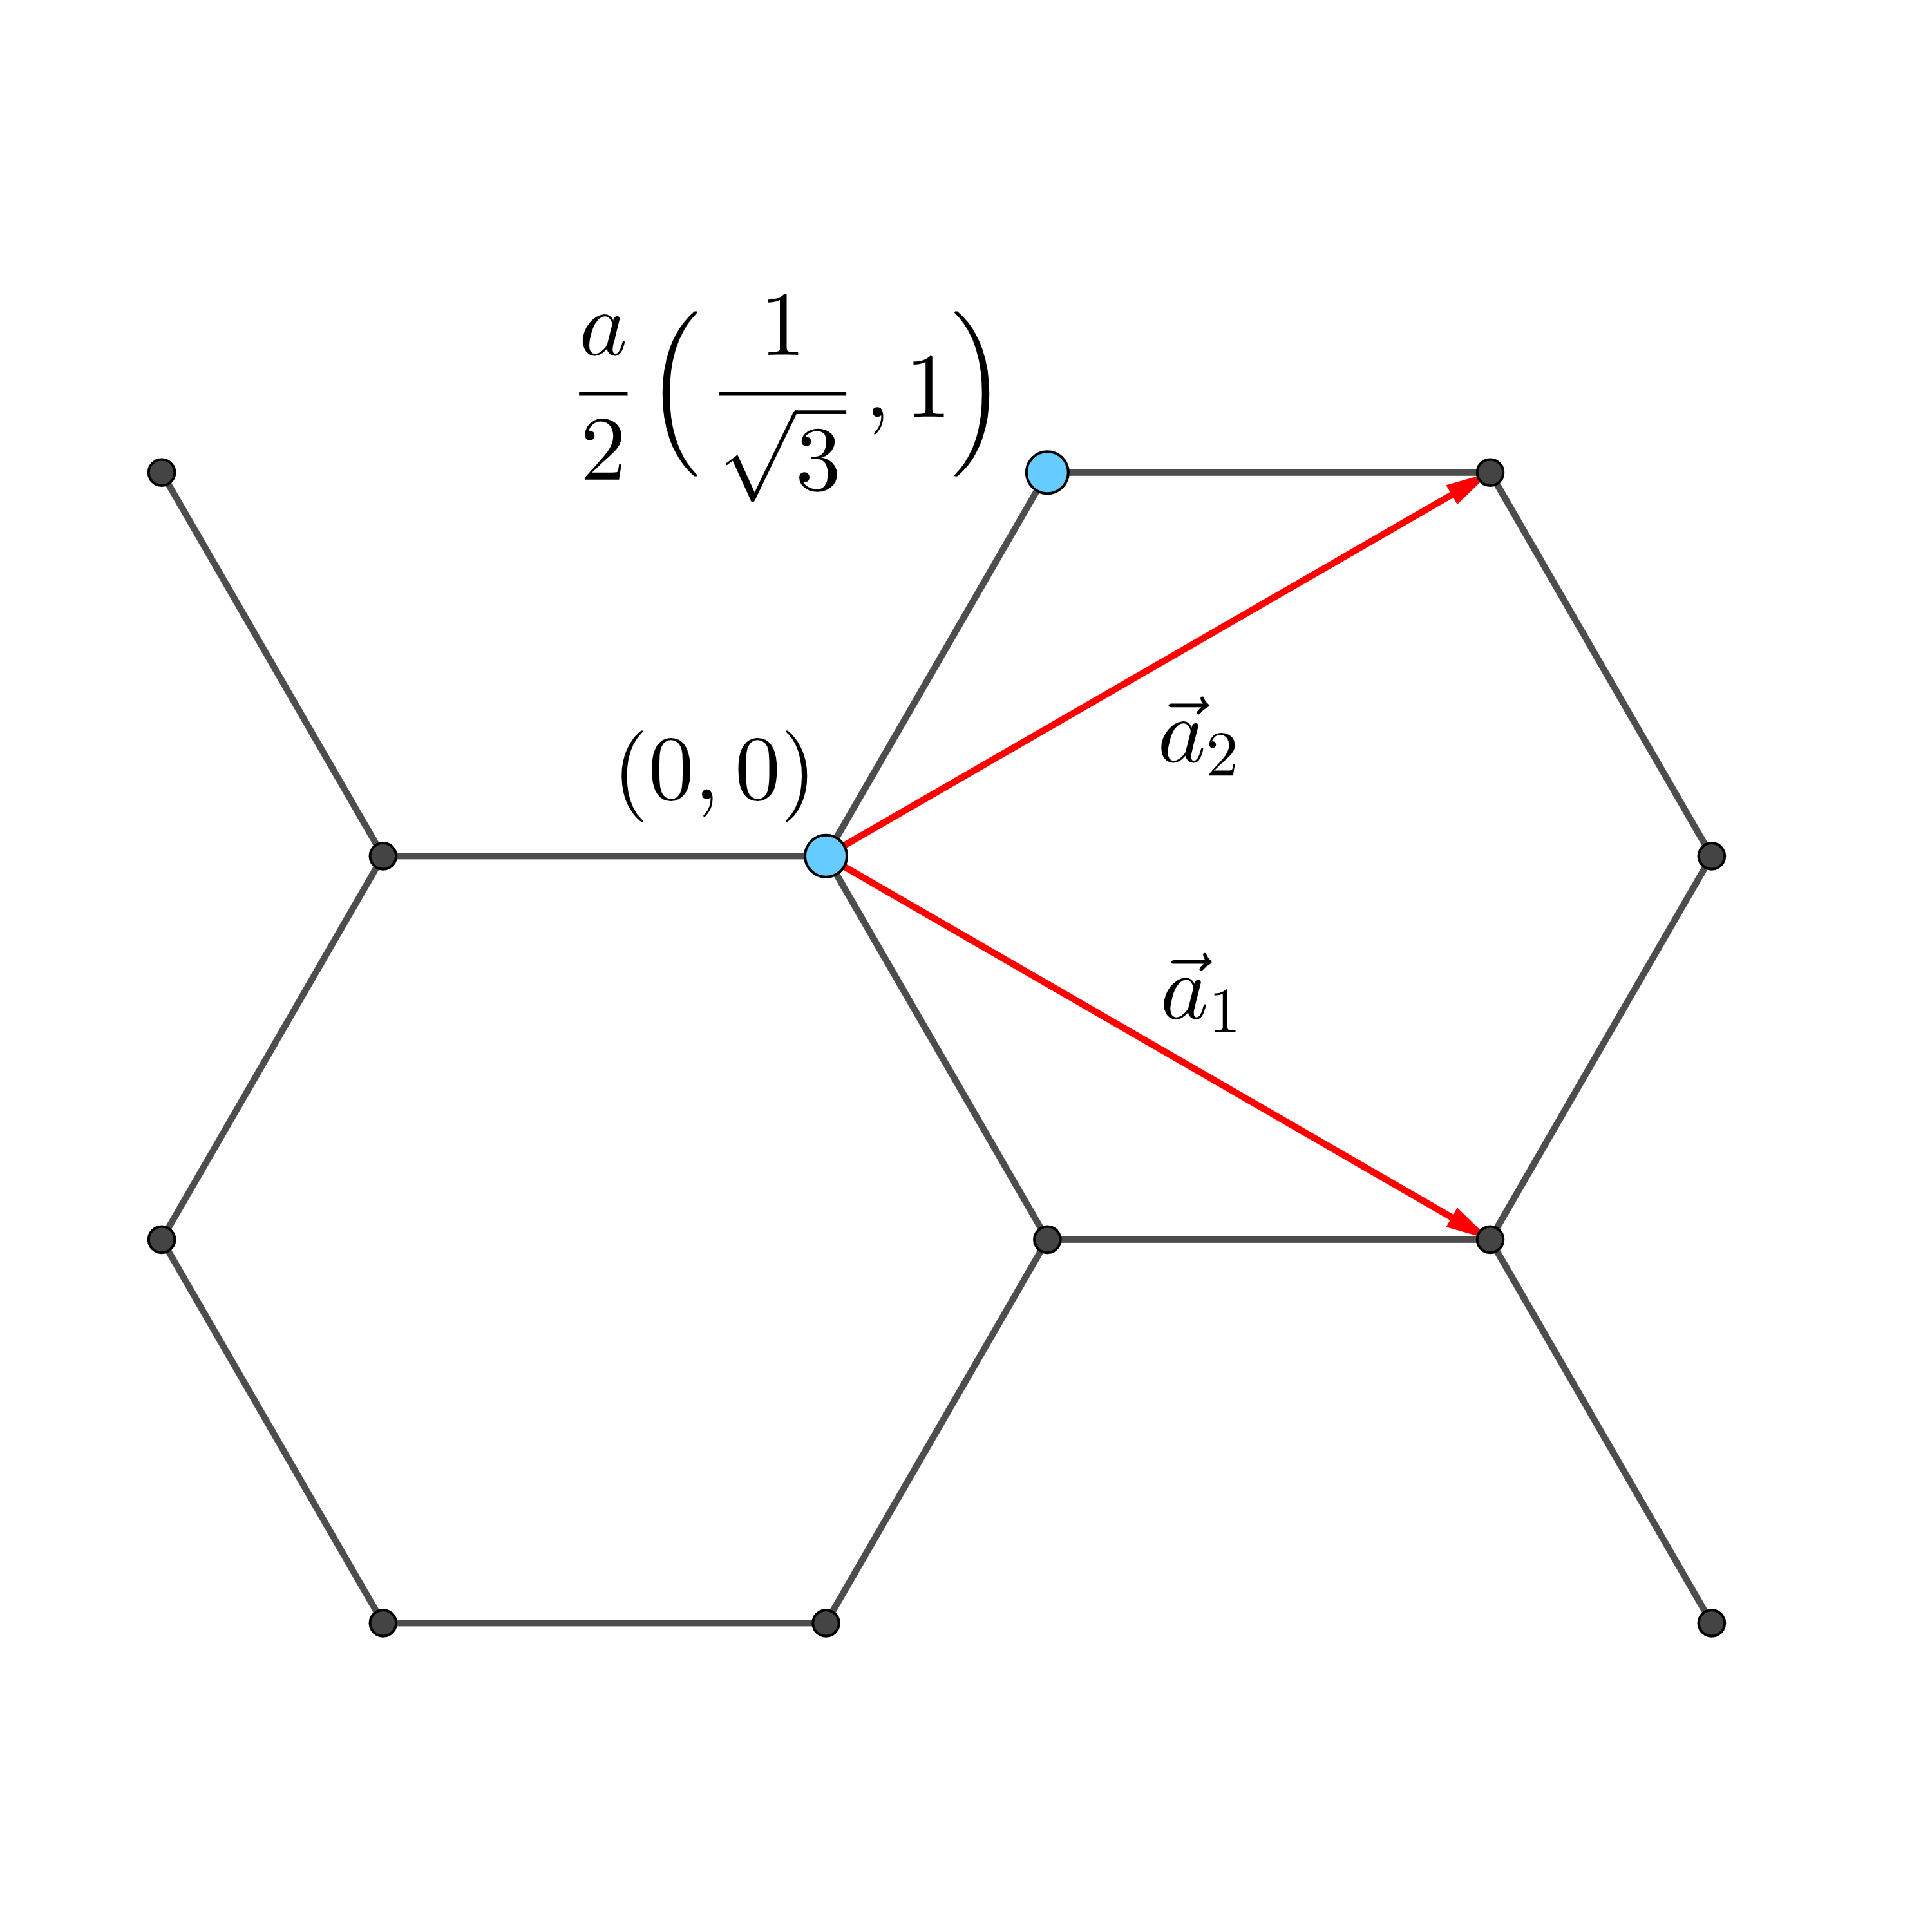
\includegraphics[width=0.70\linewidth]{../thesis/figures/system/crystal.png}
				\caption{Graphene crystal structure.}
			\end{figure}
		\end{column}%
	\end{columns}
\end{frame}
%
%%% New frame %%%
%
\begin{frame}{Creating a graphene Kirigami system}
	\framesubtitle{Sheet Kirigami}
	\begin{figure}[H]
		\centering
		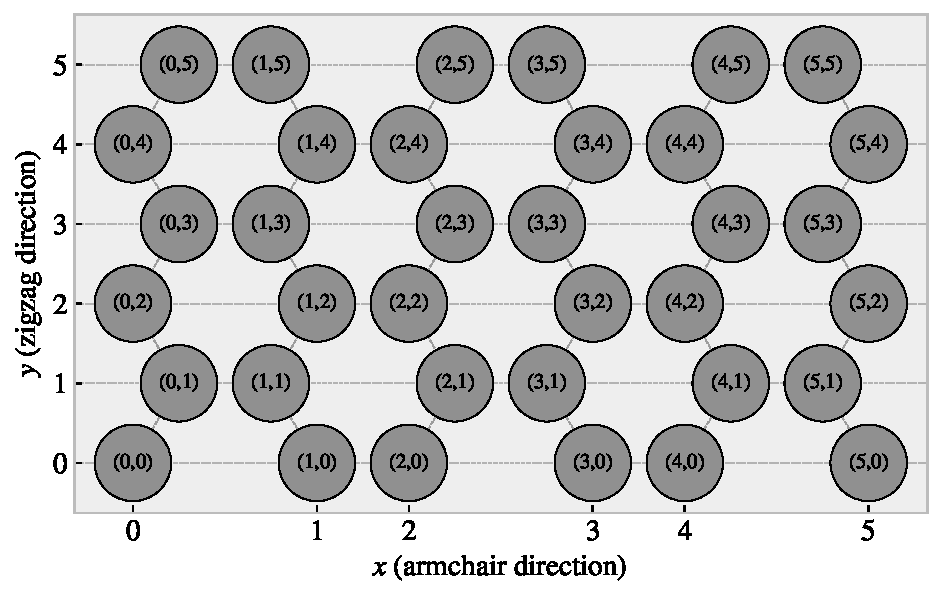
\includegraphics[width=0.7\linewidth]{../thesis/figures/system/atom_indexing.pdf}
		\caption{Graphene atom site indexing.}
	\end{figure}	
\end{frame}
%
%%% New frame %%%
%
\begin{frame}{Creating a graphene Kirigami system}
	\framesubtitle{Sheet Kirigami}
	\begin{figure}[H]
		\centering
		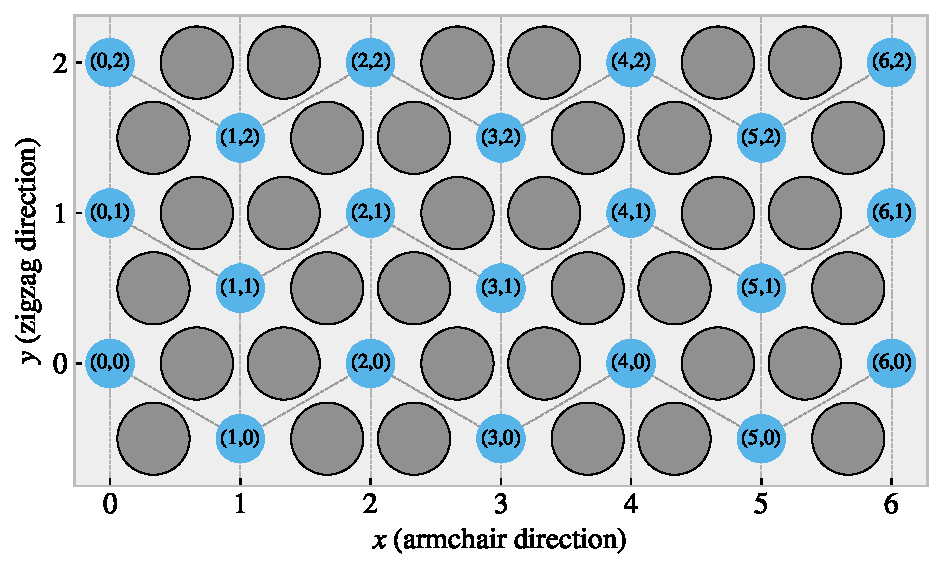
\includegraphics[width=0.7\linewidth]{../thesis/figures/system/center_indexing.pdf}
		\caption{Graphene center element indexing.}
	\end{figure}	
\end{frame}
%
%%% New frame %%%
%
\begin{frame}{Creating a graphene Kirigami system}
	\framesubtitle{Sheet Kirigami}
	\begin{figure}[H]
		\centering
		\begin{subfigure}[t]{0.48\textwidth}
			\centering
			\includegraphics[width=\textwidth]{../thesis/figures/system/pop_up_inspiration.png}
			\caption{Tetrahedron: Alternating perpendicular cuts producing a tetrahedron-shaped surface buckling when stretched. Reproduced from~\cite{new_pop_up}. }
		\end{subfigure}
		\hfill
		\begin{subfigure}[t]{0.48\textwidth}
			\centering
			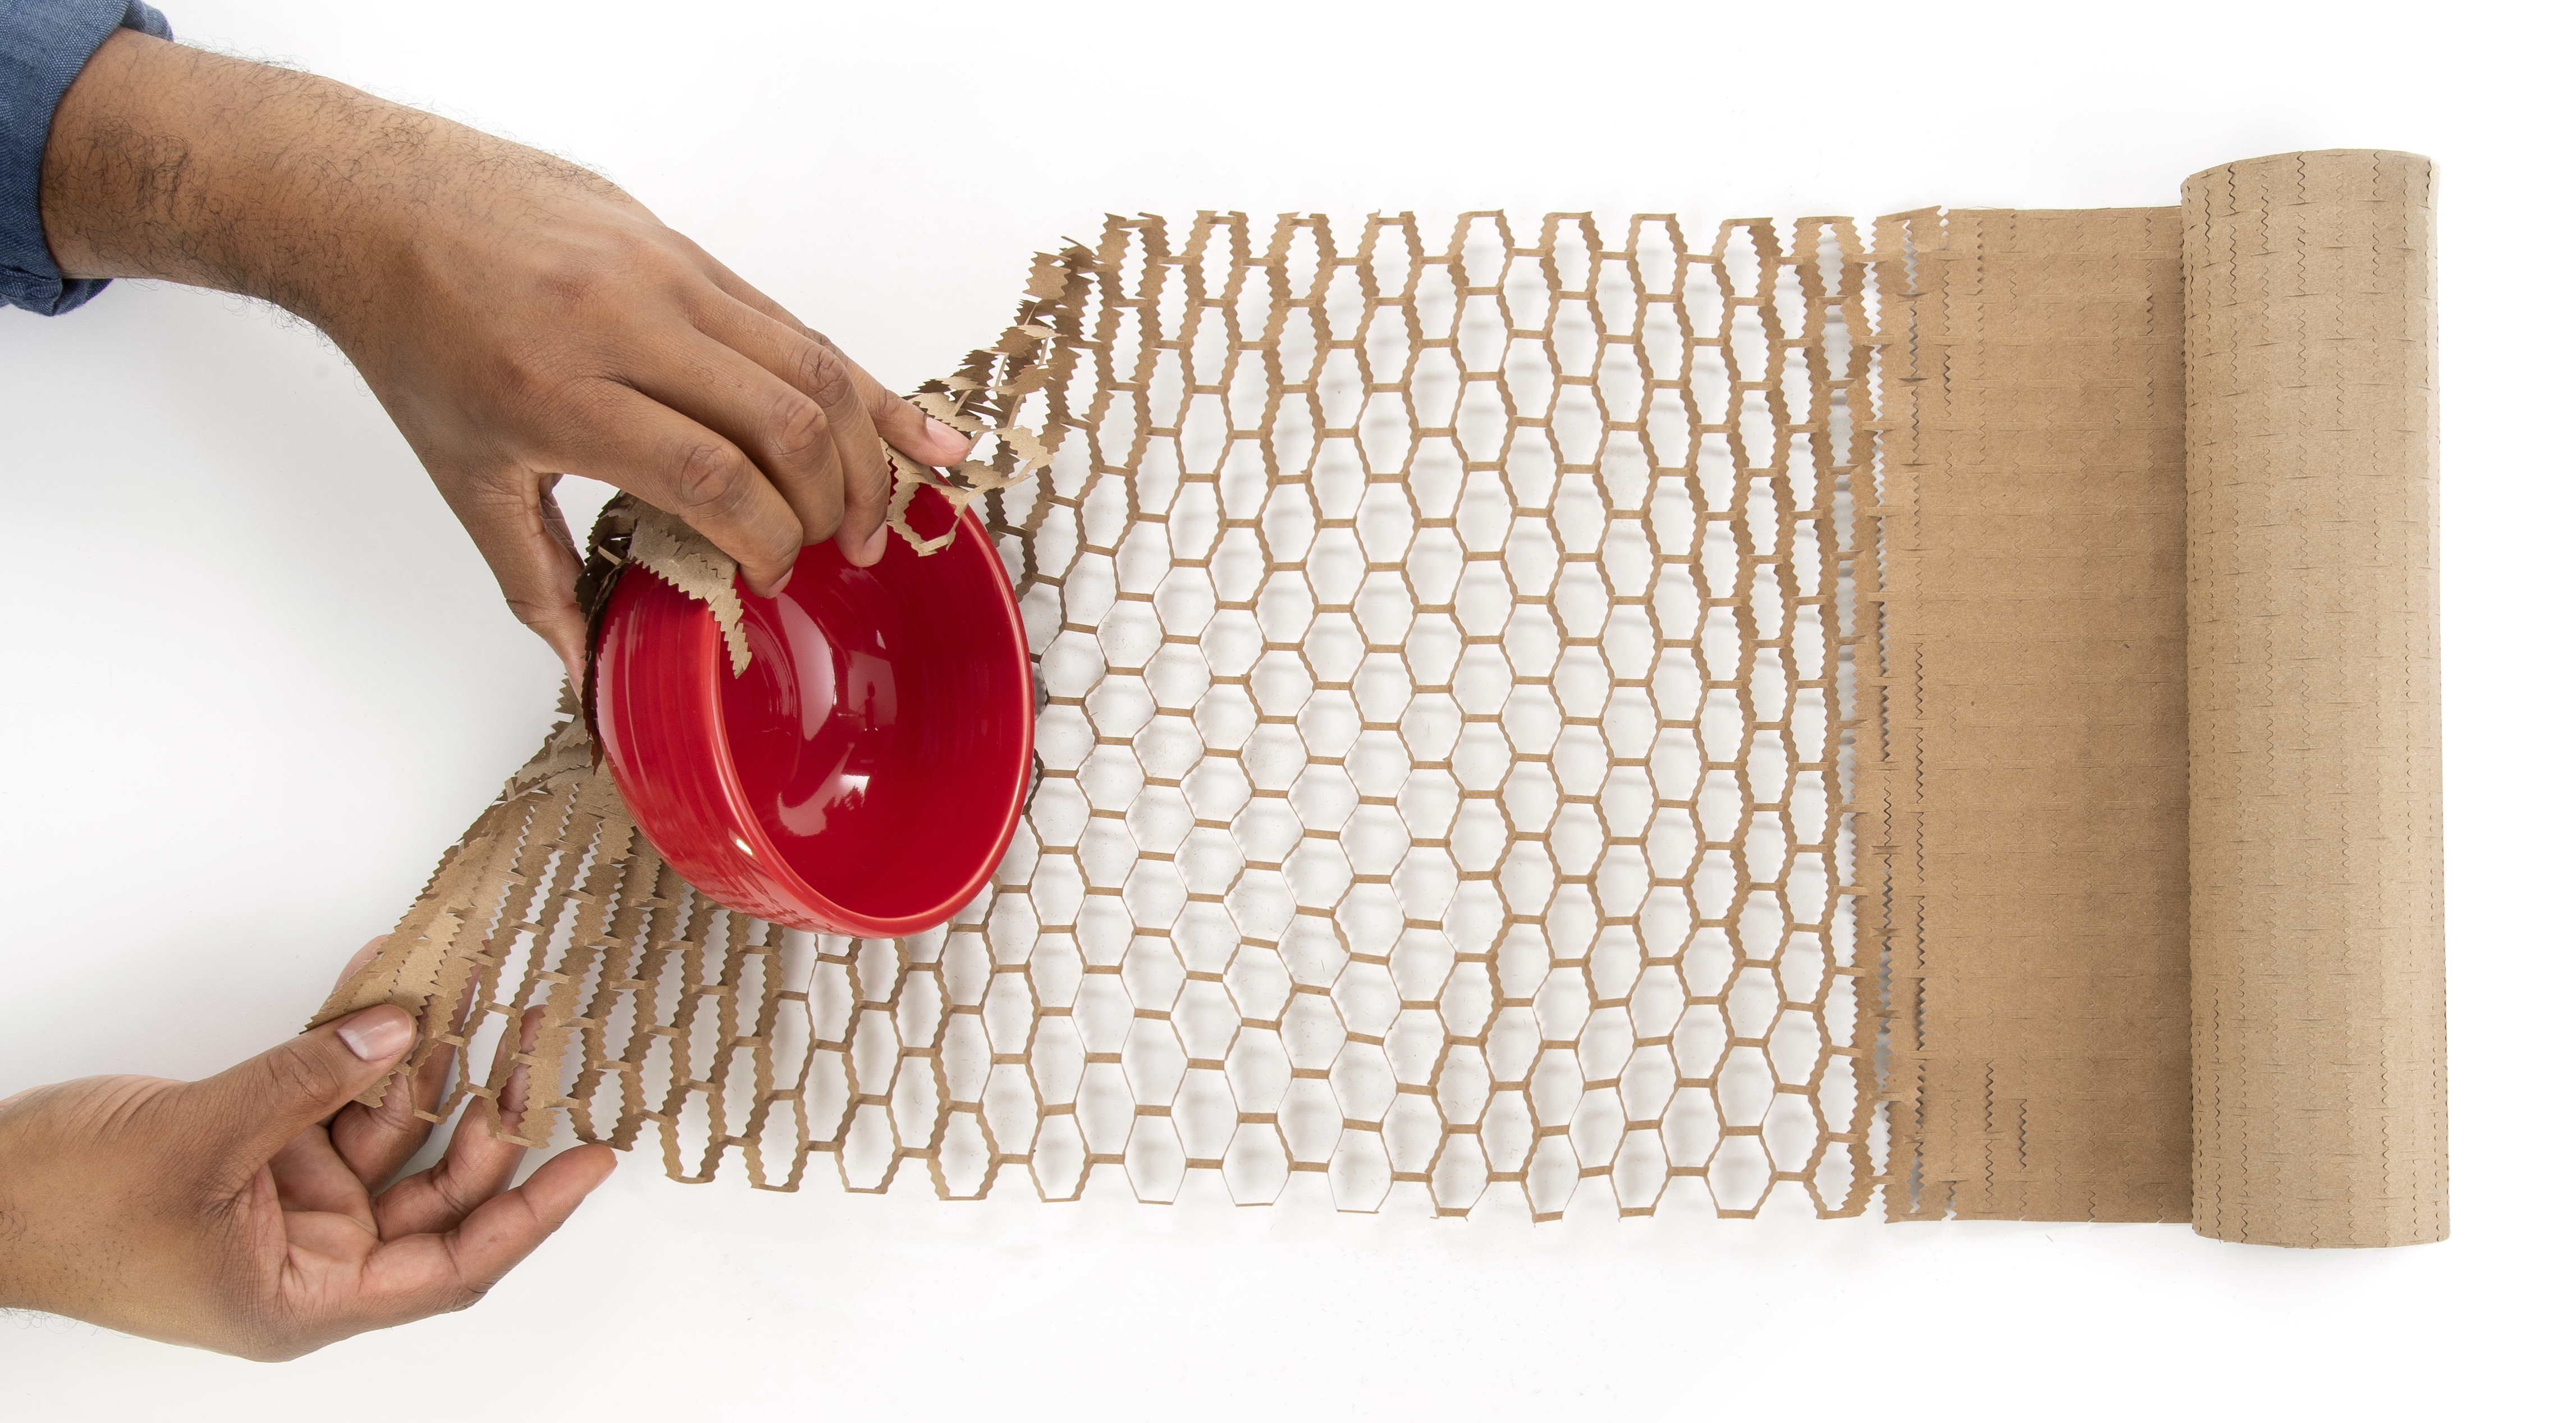
\includegraphics[width=\textwidth]{../thesis/figures/system/honeycomb_inspiration.jpg}
			\caption{Honeycomb: Scotch\textsuperscript{TM} Cushion Lock\textsuperscript{TM}~\cite{cushion_wrap} producing a honeycomb-shaped surface buckling when stretched. Reproduced from~\cite{cushion_wrap}.}
		\end{subfigure}
		\hfill
		\caption{Macroscale kirigami cut patterns used as inspiration for the nanoscale implementation.}
	  \end{figure}
\end{frame}
%
%%% New frame %%%
%
\begin{frame}{Creating a graphene Kirigami system}
	\framesubtitle{Sheet Kirigami}
	

	\begin{figure}[H]
		\centering
		\begin{subfigure}[t]{0.49\textwidth}
			\centering
			\raggedleft
			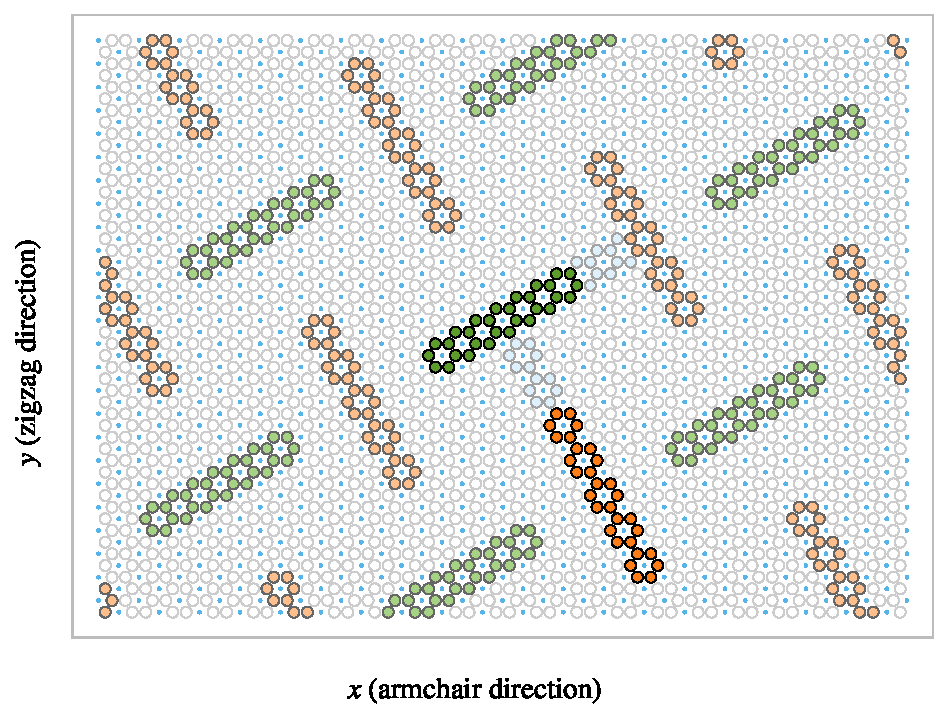
\includegraphics[width=0.7\textwidth]{../thesis/figures/system/pop_up_inverse.pdf}
			% \caption{}
		  \end{subfigure}
		  \hfill
		  \begin{subfigure}[t]{0.49\textwidth}
			\centering
			\raggedright
			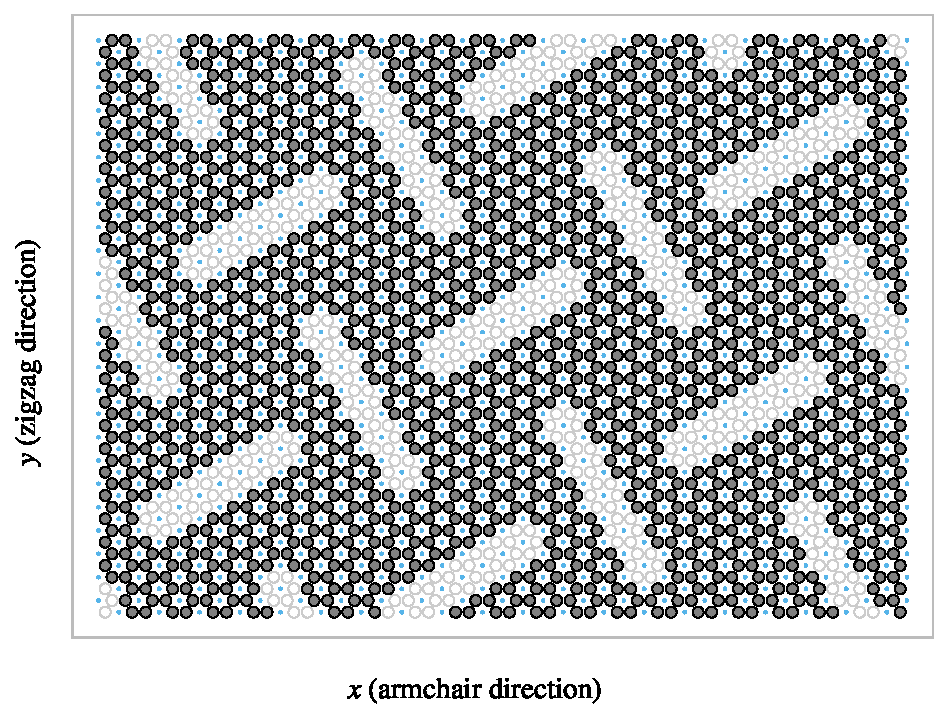
\includegraphics[width=0.7\textwidth]{../thesis/figures/system/pop_up_pattern.pdf}
			% \caption{}
		\end{subfigure}

	  \end{figure}
	  
	  
	  \begin{figure}[H]
		\centering
		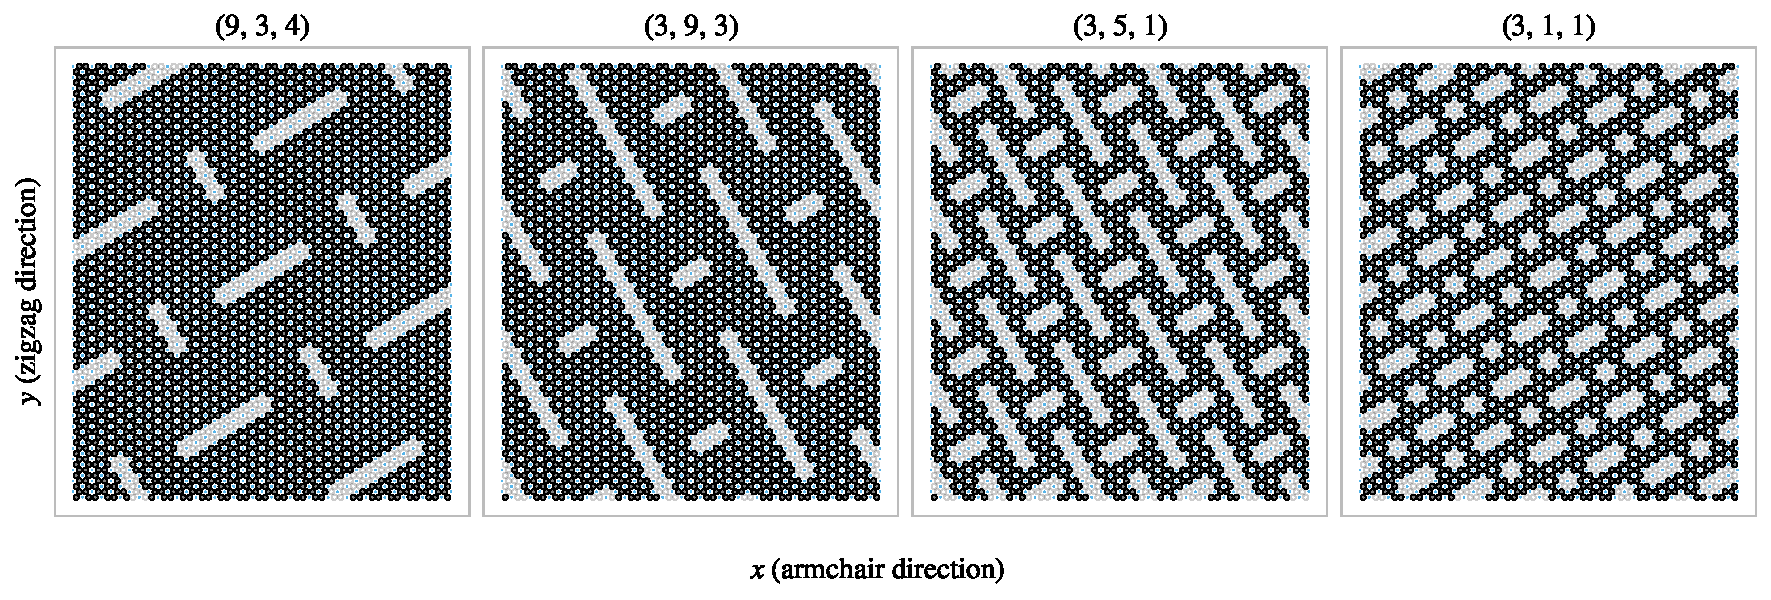
\includegraphics[width=\linewidth]{../thesis/figures/system/pop_up_flavors.pdf}
	  \end{figure}
	  
\end{frame}
%
%%% New frame %%%
%
\begin{frame}{Creating a graphene Kirigami system}
	\framesubtitle{Sheet Kirigami}


	\begin{figure}[H]
		\centering
		\begin{subfigure}[t]{0.48\textwidth}
			\centering
			\raggedleft
			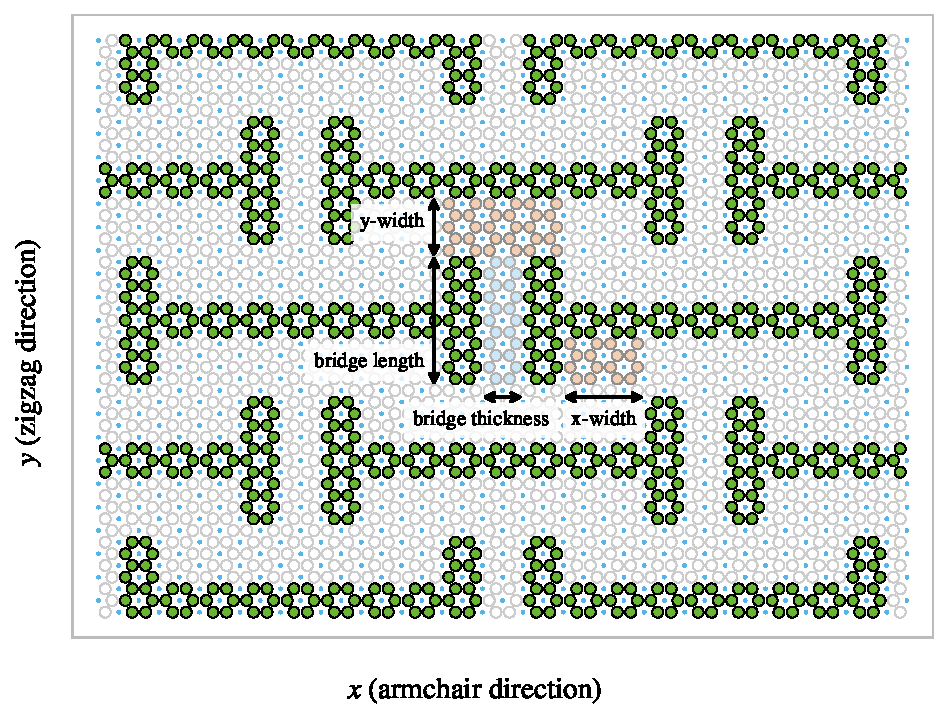
\includegraphics[width=0.7\textwidth]{../thesis/figures/system/honeycomb_inverse.pdf}
		  \end{subfigure}
		  \hfill
		  \begin{subfigure}[t]{0.48\textwidth}
			\centering
			\raggedright
			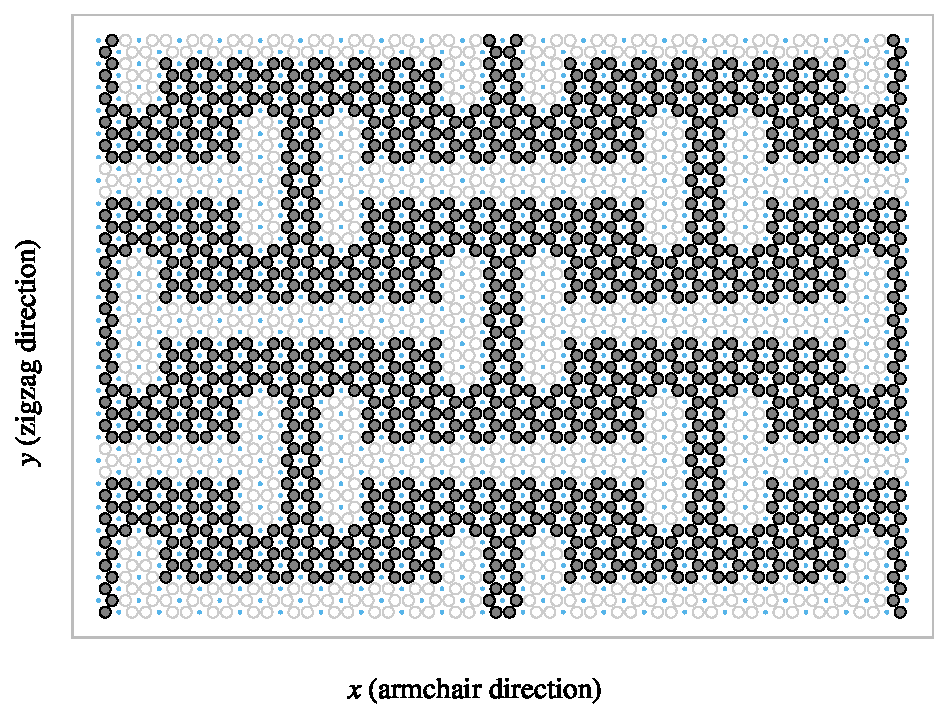
\includegraphics[width=0.7\textwidth]{../thesis/figures/system/honeycomb_pattern.pdf}
		\end{subfigure}
	  \end{figure}
	  
	  
	  \begin{figure}[H]
		\centering
		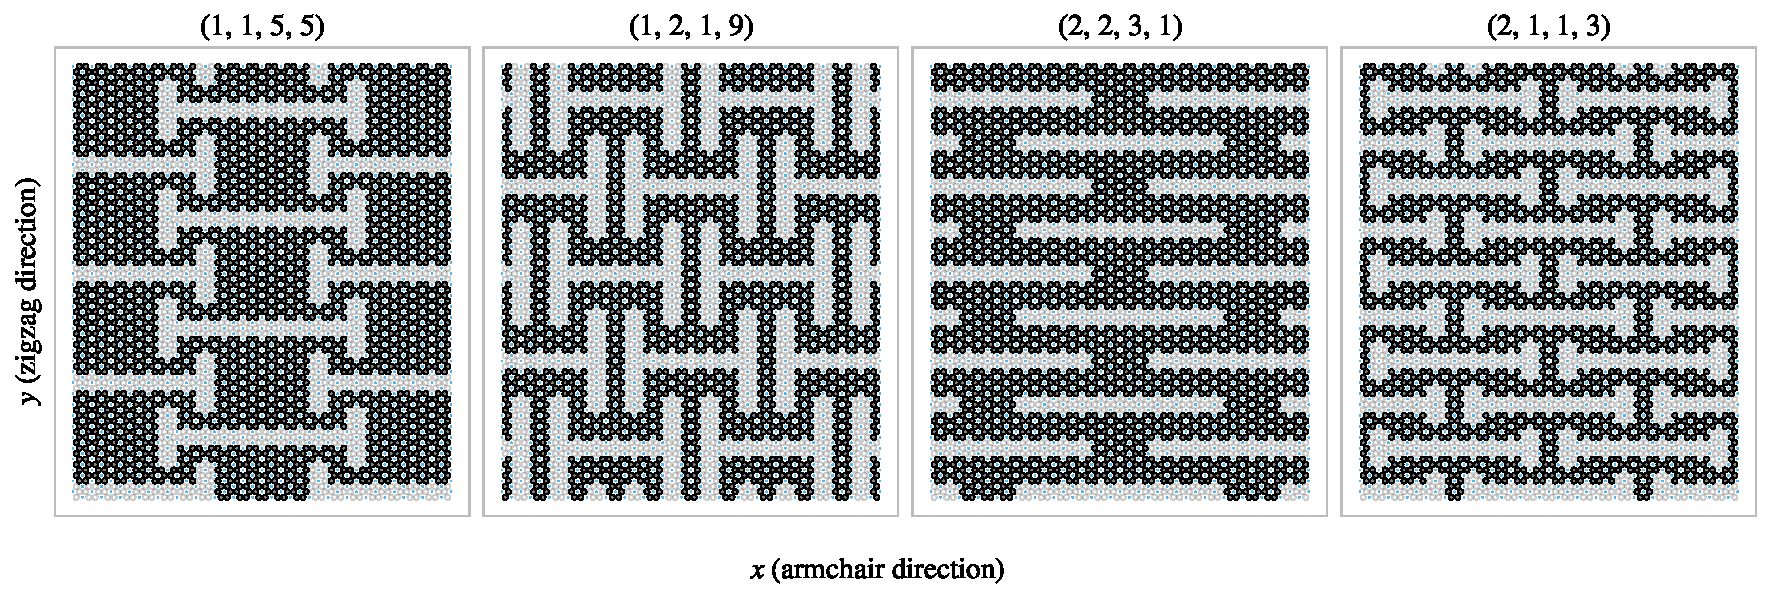
\includegraphics[width=\linewidth]{../thesis/figures/system/honeycomb_flavors.pdf}
	  \end{figure}
\end{frame}
%
%%% New frame %%%
%
\begin{frame}{Creating a graphene Kirigami system}
	\framesubtitle{Sheet Kirigami}
	Random walk 
	\begin{figure}[H]
		\centering
		\includegraphics[width=0.8\linewidth]{../thesis/figures/system/RW_flavors.png}
	\end{figure}
\end{frame}
%
%%% New frame %%%
%
\begin{frame}{Creating a graphene Kirigami system}
	\framesubtitle{MD simulation}
	Introduction to MD simulation. Something about newtons equations and Langevin maybe?
\end{frame}


\section{Pilot study} %%%%%%%%%%%%%%%%%%%%%%%%%%%%%%%%%%%%%%%%%%%%%%%%%%%%%%%%%%%%%
\begin{frame}{Outline}
    \tableofcontents[currentsection]
\end{frame}

\subsection{Friction metrics}
\begin{frame}{Pilot study}
	\framesubtitle{Friction metrics}

	\begin{itemize}
		\item Friction metrics?
		\item Stick slip?
	\end{itemize}
\end{frame}
%
%%% New frame %%%
%

\subsection{Out-of-plane buckling}
\begin{frame}{Pilot study}
	\framesubtitle{Out-of-plane buckling}
	\begin{figure}
		\centering    
		\movie[open]{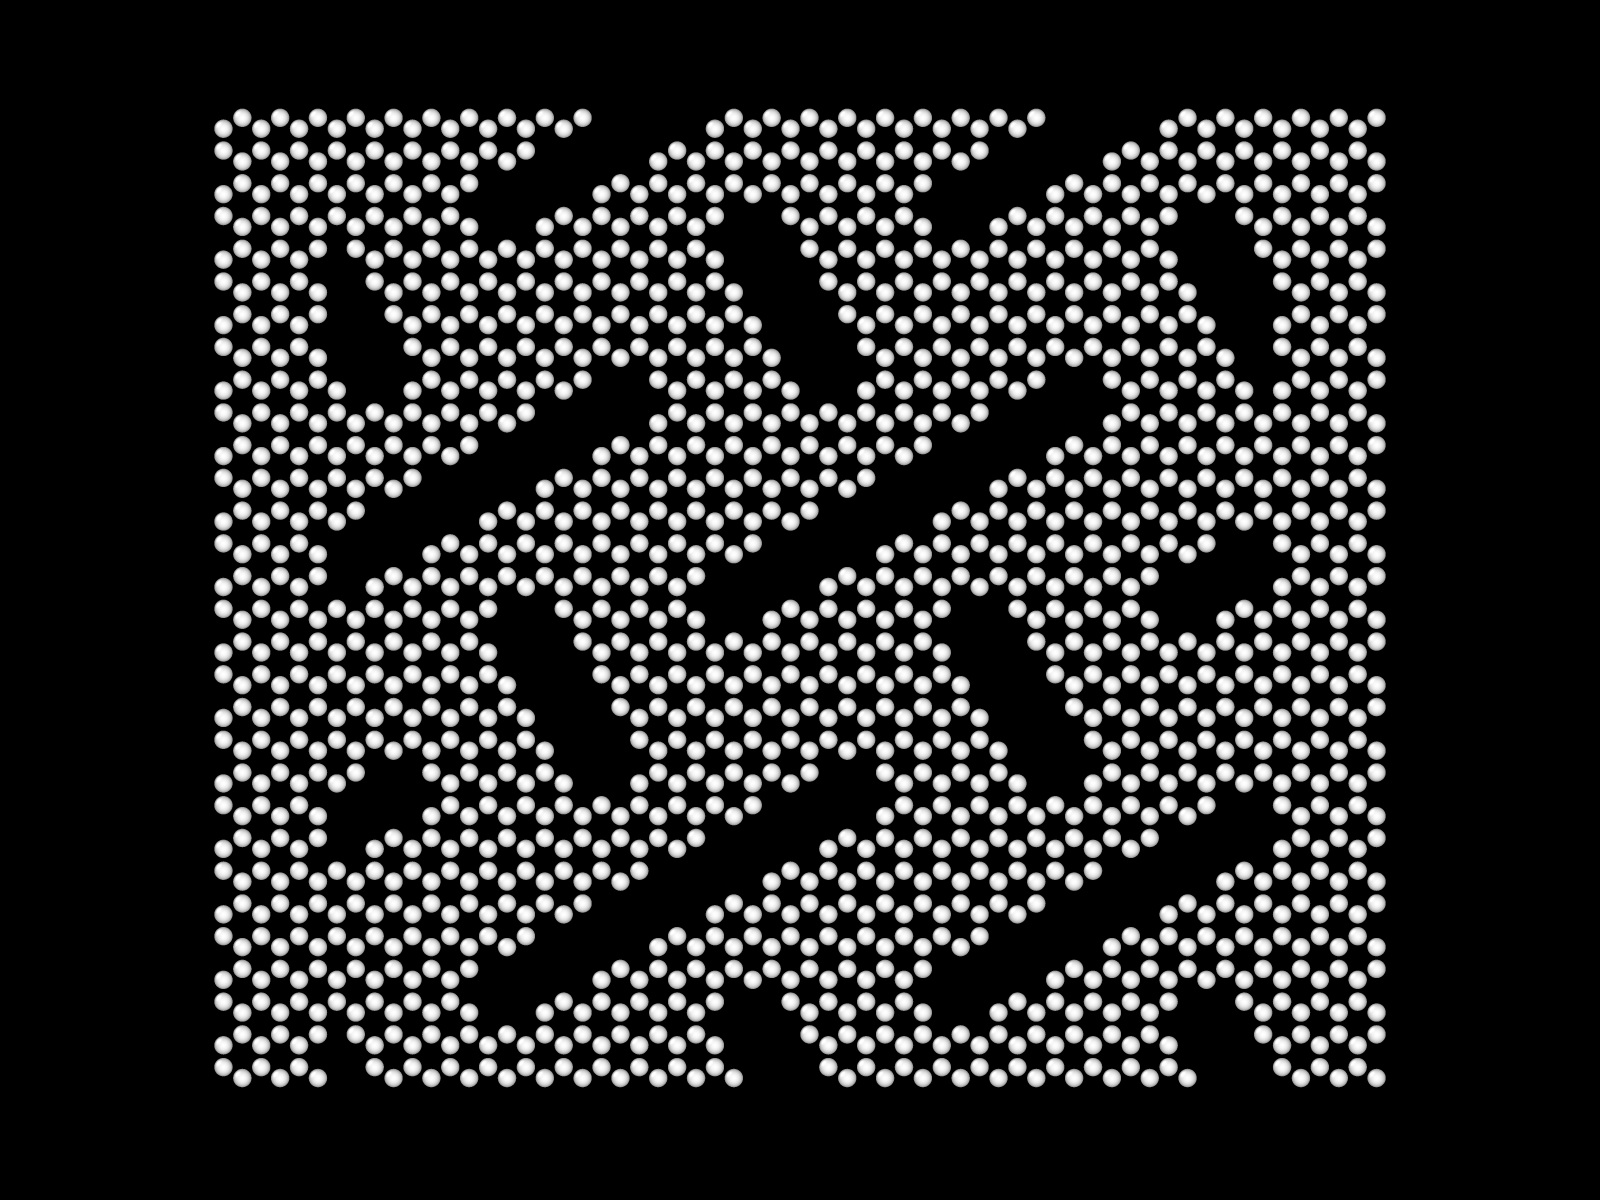
\includegraphics[height=0.7\textheight, keepaspectratio]{figures/vacuum_stretch.png}}{figures/vacuum_stretch.mov}
		\caption{Kirigami sheet stretch in vacuum. Small tetrahedron pattern.}
	\end{figure} 

\end{frame}
%
%%% New frame %%%
%
\begin{frame}{Pilot study}
	\framesubtitle{Out-of-plane buckling}
	\begin{figure}
		\centering    
		\movie[open]{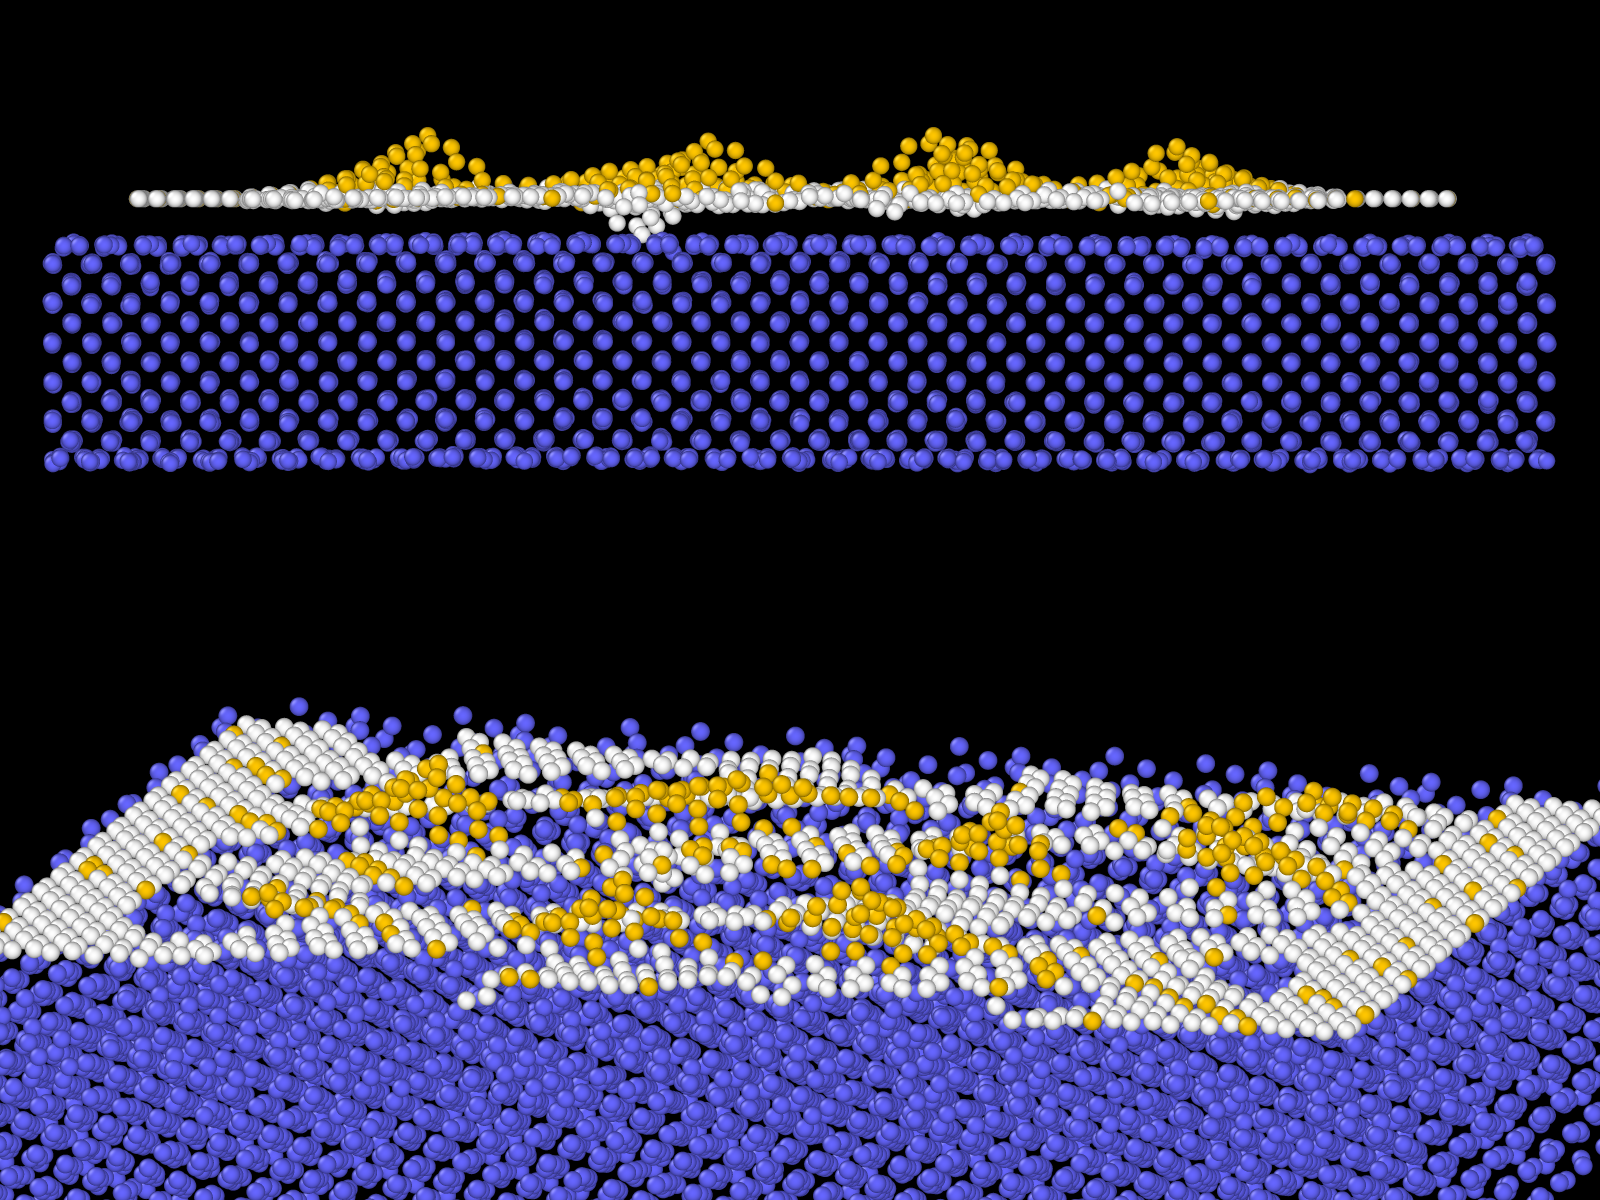
\includegraphics[height=0.7\textheight, keepaspectratio]{figures/contact_stretch.png}}{figures/contact_stretch.mov}
		\caption{Kirigami stretch in contact with Si-substrate.}
	\end{figure} 
\end{frame}
%
%%% New frame %%%
%
\begin{frame}{Pilot study}
	\framesubtitle{Out-of-plane buckling}
	\begin{figure}
		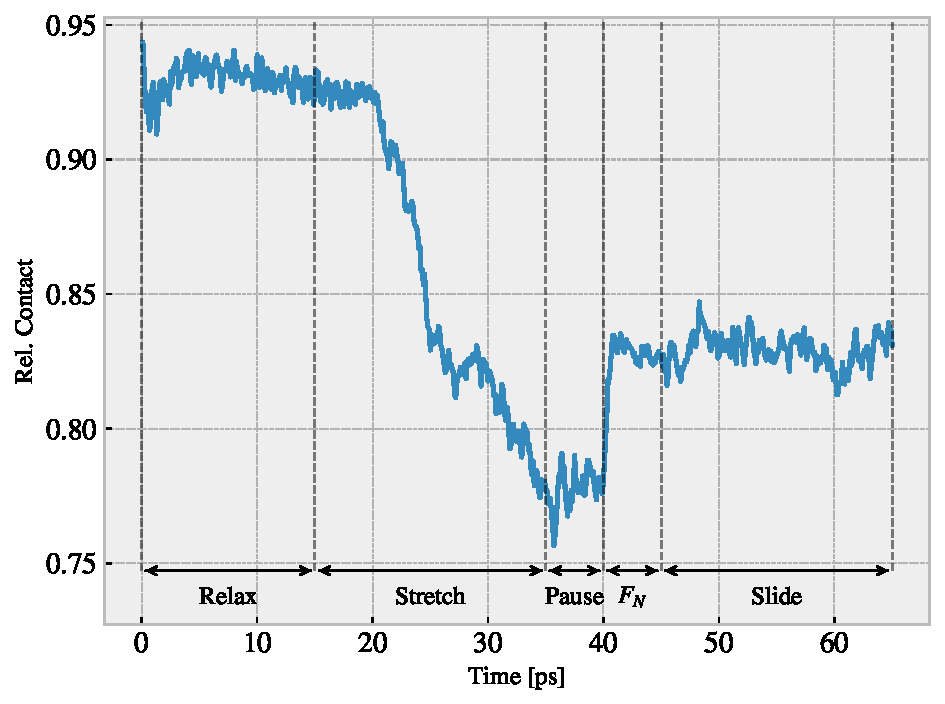
\includegraphics[height=0.7\textheight]{figures/contact_pct.pdf}
		\caption{Contact area approximation: Number of C-Si bonds within a threshold distance of 110\% the LJ interaction equilibrium distance.}
	\end{figure}	
\end{frame}
%
%%% New frame %%%
%
\begin{frame}{Pilot study}
	\framesubtitle{Out-of-plane buckling}
	\begin{figure}[H]
		\centering
		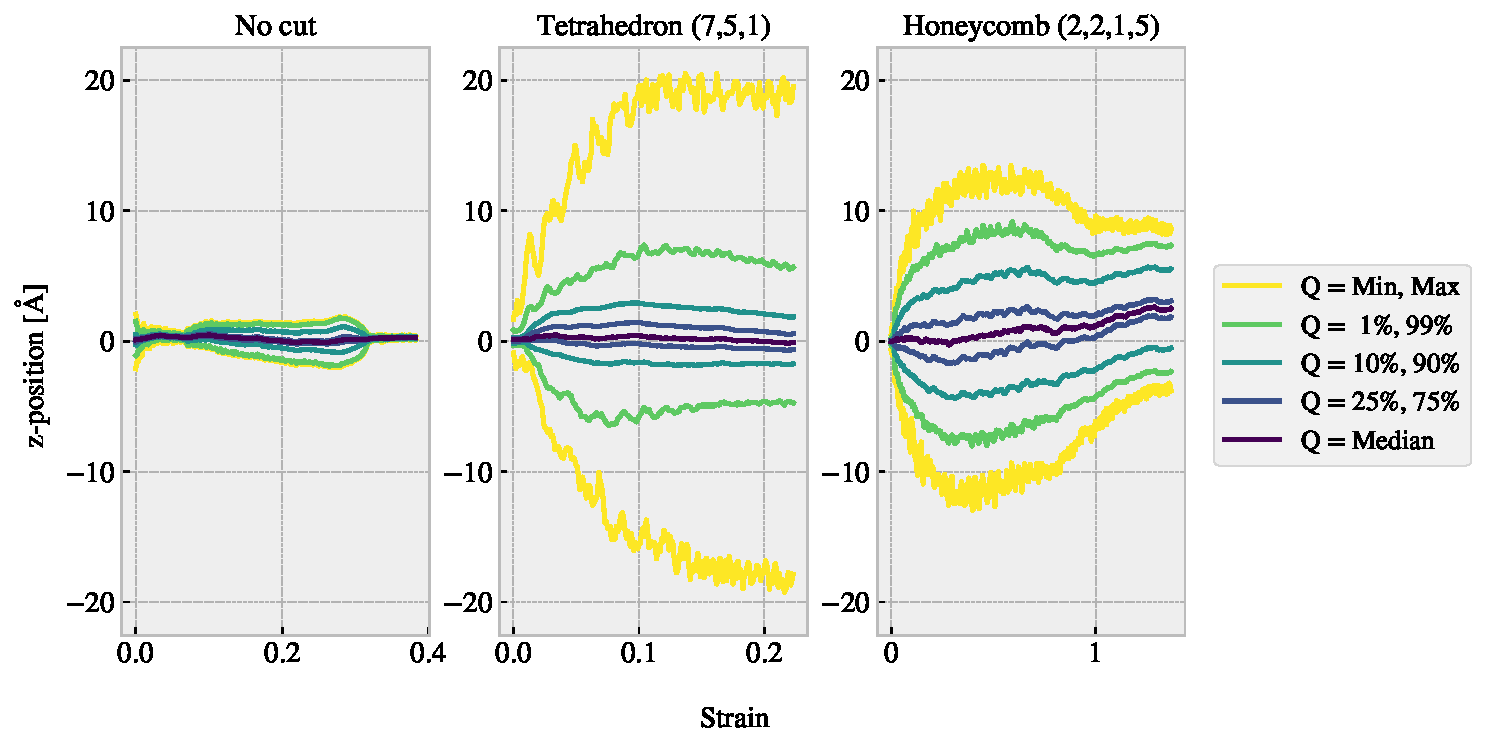
\includegraphics[width=\linewidth]{../thesis/figures/baseline/vacuum_normal_buckling.pdf}
		% \caption{The out-of-plane buckling during straining for the non-cut (No cut), Tetrahedron $(7,5,1)$, and Honeycomb $(2,2,1,5)$ pattern respectively in vacuum at low temperature $T = \SI{5}{K}$. The buckling is quantified by the distribution of the atom z-positions, which are perpendicular to the sheet plane, and the colors indicate selected quantiles. The rupture strain for each pattern, from left to right, is 0.38, 0.22, and 1.37, respectively. The results indicate that the Tetrahedron and Honeycomb patterns exhibit significant out-of-plane buckling in comparison to the non-cut sheet.}
		% \label{fig:buckling_quartiles}
	 \end{figure}
\end{frame}
%
%%% New frame %%%
%
\begin{frame}{Pilot study}
	\framesubtitle{Out-of-plane buckling}
	\begin{figure}[H]
		\centering
		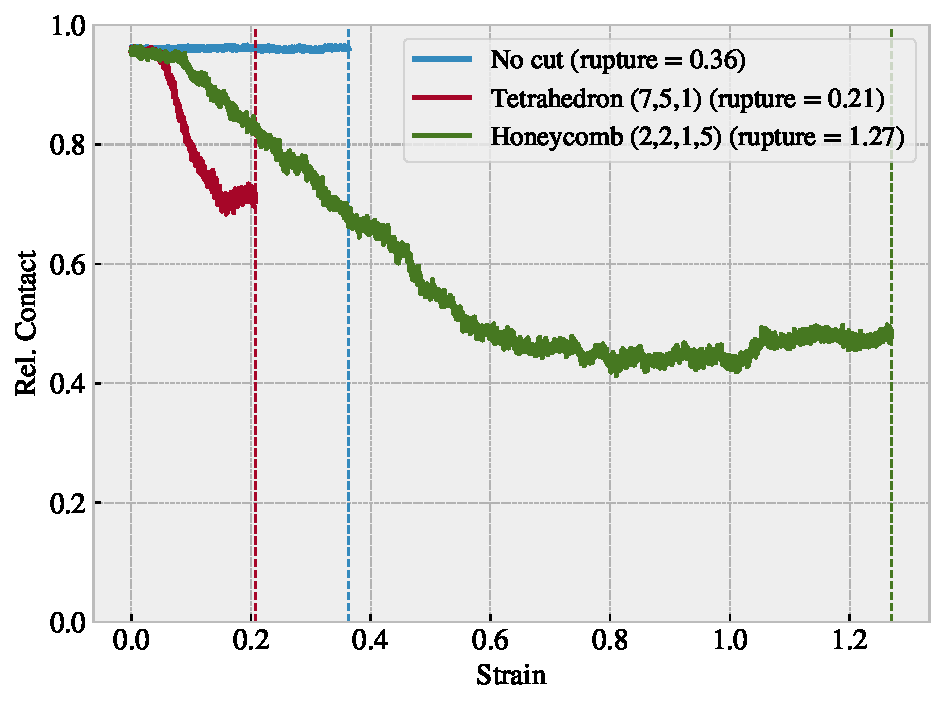
\includegraphics[width=0.5\linewidth]{../thesis/figures/baseline/contact_vs_stretch.pdf}
		% \caption{The relative contact during straining of the non-cut (No cut), Tetrahedron $(7,5,1)$, and Honeycomb $(2,2,1,5)$ pattern respectively in contact with a substrate. The relative contact is given as the relative number of atoms in the sheet within chemical interaction range. The cut-off for the interaction range is \SI{4}{\text{Å}} corresponding to $\sim 120 \%$ the \acrshort{LJ} equilibrium distance. No normal force is applied and the temperature is kept at $T = \SI{300}{K}$.}
		% \label{fig:contact_vs_stretch}
	\end{figure}
\end{frame}
%
%%% New frame %%%
%



\subsection{Friction-strain profiles}
\begin{frame}{Pilot study}
	\framesubtitle{Friction-strain profiles}

	\begin{figure}[H]
		\centering
		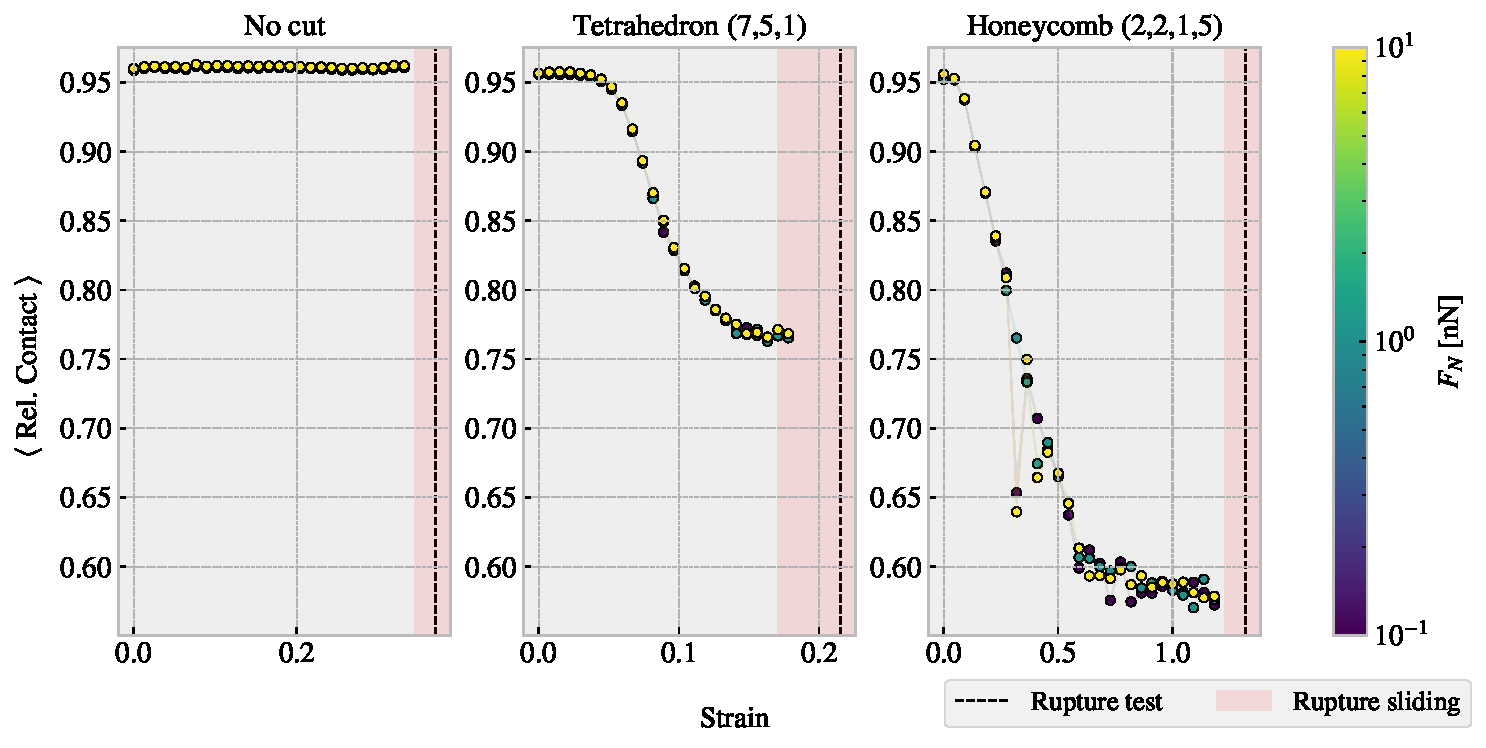
\includegraphics[width=1\linewidth]{../thesis/figures/baseline/multi_stretch_area_compare.pdf}
	\end{figure}
\end{frame}
%
%%% New frame %%%
%
\begin{frame}{Pilot study}
	\framesubtitle{Friction-strain profiles}

	\begin{figure}[H]
		\centering
		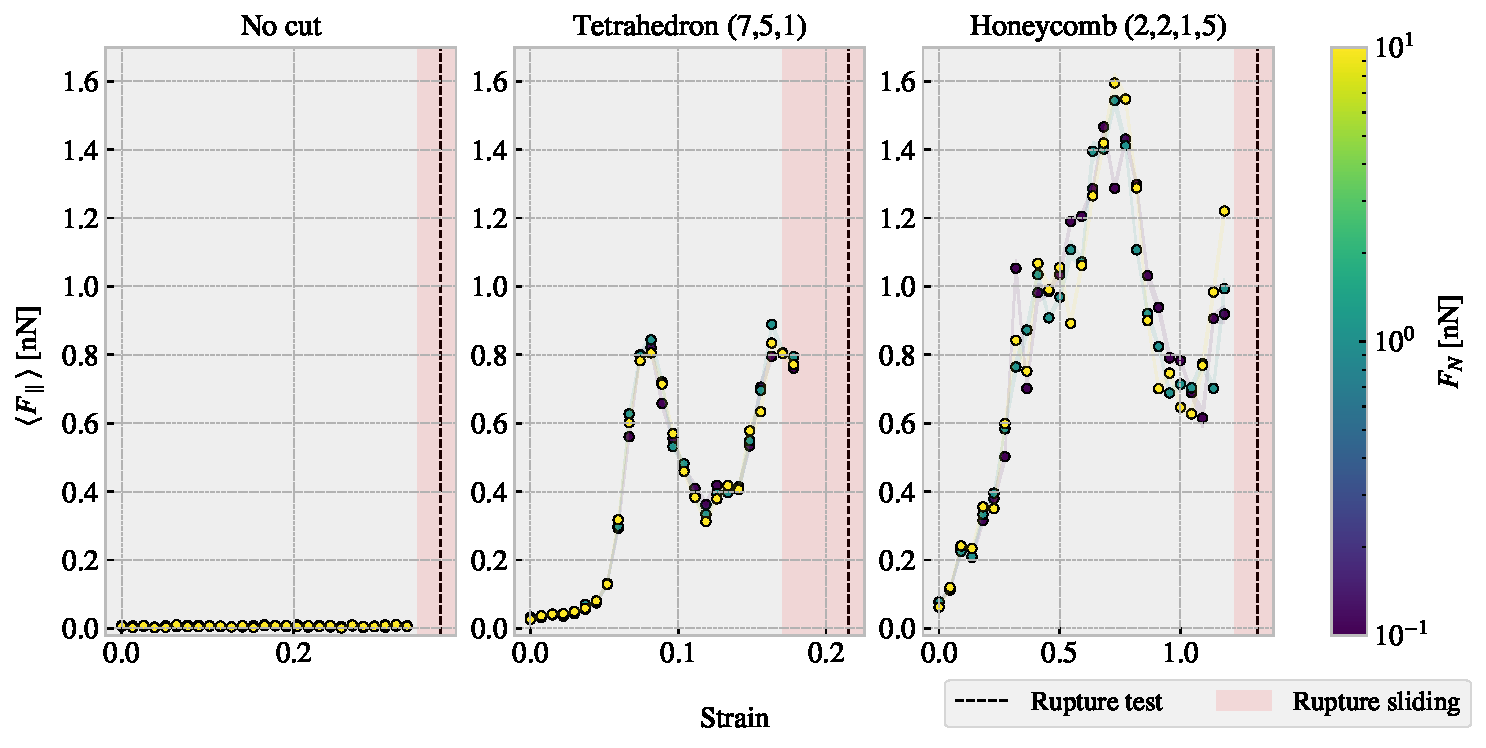
\includegraphics[width=1\linewidth]{../thesis/figures/baseline/multi_stretch_mean_compare.pdf}
	\end{figure}
\end{frame}
%
%%% New frame %%%
%
\subsection{Negative friction coefficient}
\begin{frame}{Pilot study}
	\framesubtitle{Negative friction coefficient}
	Load to sheet tension coupling 
	\begin{align*}
		F_t = TF_N, \qquad T = 6
	\end{align*}
	\begin{figure}[H]
		\centering
		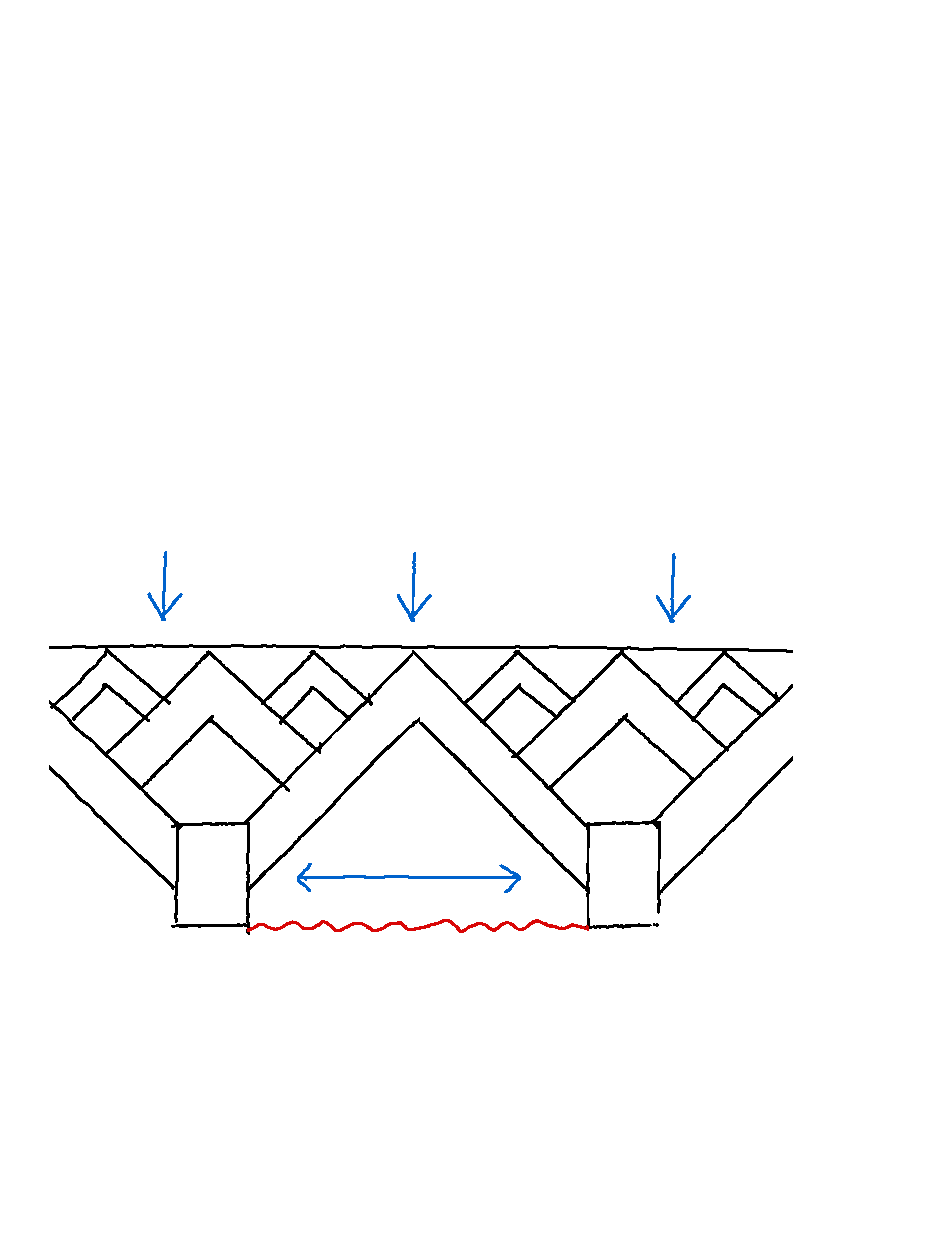
\includegraphics[width=0.6\linewidth]{../thesis/figures/negative_coefficient/nanomachine.pdf}
		% \caption{Working sketch for a nanomachine design that aims to translate applied load (from the top of the figure) to a straining of the graphene sheet (shown in red). The black boxes connected to the graphene sheet represent the pull blocks in our system.}
		% \label{fig:nanomachine}
	\end{figure}	  
\end{frame}
%
%%% New frame %%%
%
\begin{frame}{Pilot study}
	\framesubtitle{Negative friction coefficient}

	\begin{figure}[H]
		\centering
		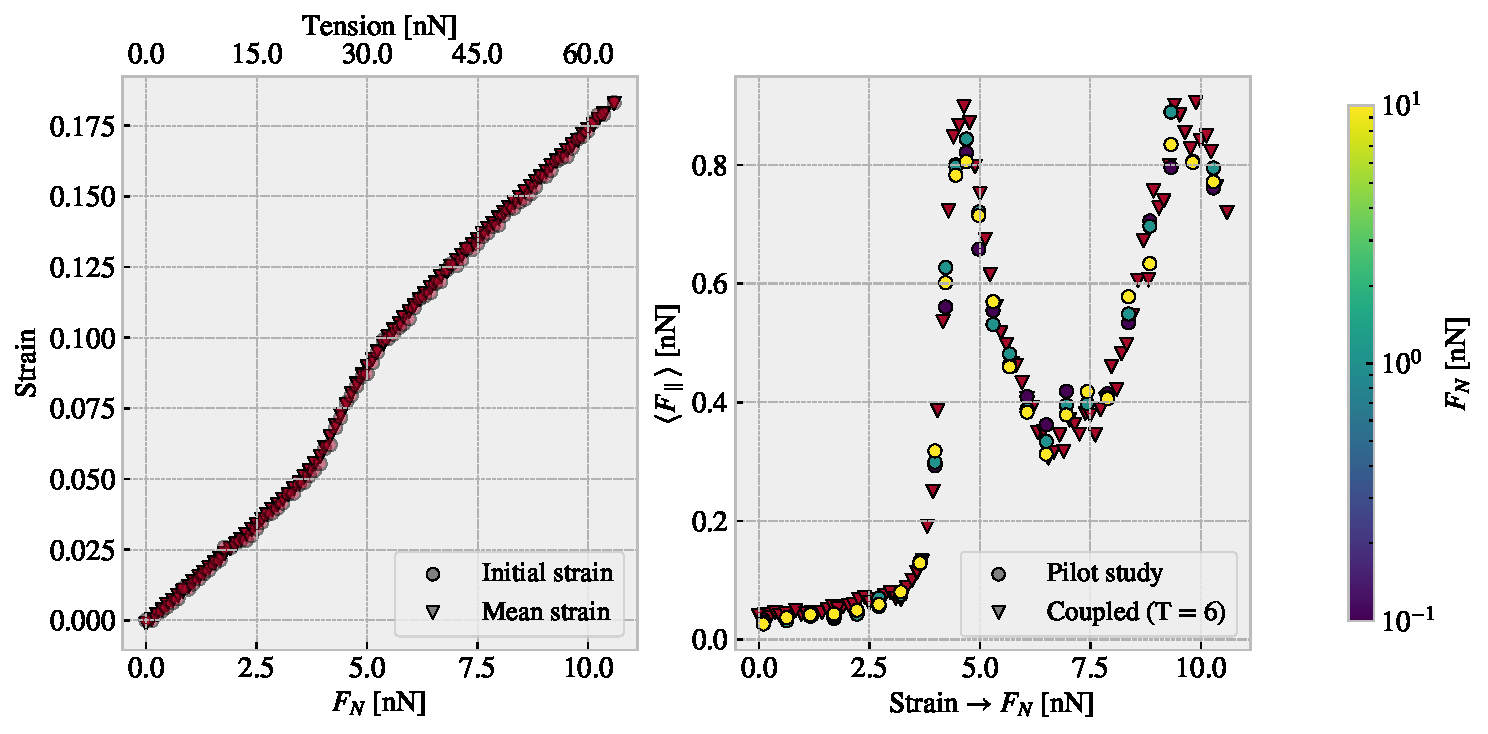
\includegraphics[width=\linewidth]{../thesis/figures/negative_coefficient/manual_coupling_tension_pop7_5_1.pdf}	
		\caption{Tetrahedron $(7,5,1)$}
	\end{figure}	
\end{frame}
%
%%% New frame %%%
%

\begin{frame}{Pilot study}
	\framesubtitle{Negative friction coefficient}

	\begin{figure}[H]
		\centering
		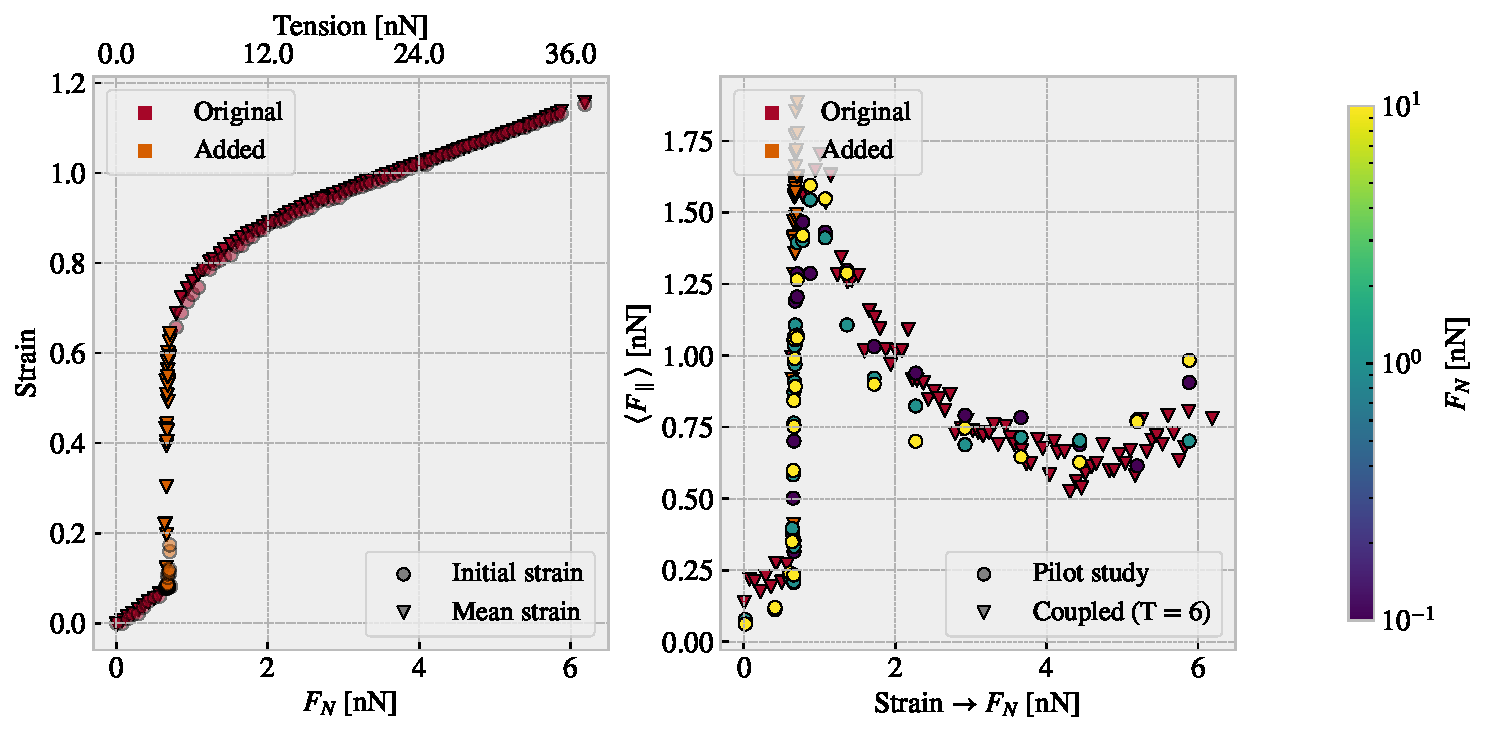
\includegraphics[width=\linewidth]{../thesis/figures/negative_coefficient/manual_coupling_tension_hon2215.pdf}	
	\caption{Honeycomb $(2,2,1,5)$}
	\end{figure}	
\end{frame}
%
%%% New frame %%%
%
\begin{frame}{Pilot study}
	\framesubtitle{Negative friction coefficient}
	Honeycomb stretch simulation topview
\end{frame}
%
%%% New frame %%%
%


\section{Kirigami configuration search} %%%%%%%%%%%%%%%%%%%%%%%%%%%%%%%%%%%%%%%%%%%%%%%%%%%%%%%%%%%%%
\begin{frame}{Outline}
    \tableofcontents[currentsection]
\end{frame}

\subsection{Machine learning}
\subsection{Accelerated search}



\section{Summary and outlook} %%%%%%%%%%%%%%%%%%%%%%%%%%%%%%%%%%%%%%%%%%%%%%%%%%%%%%%%%%%%%
\begin{frame}{Outline}
    \tableofcontents[currentsection]
\end{frame}




\begin{frame}%[allowframebreaks]
	\frametitle{References}
	\printbibliography
	% \bibliographystyle{apalike}
	% \bibliographystyle{plain}
	% \printbibliography
	% \bibliography{./presentation/bibliography.bib}
\end{frame}



\end{document} 


